\documentclass[a4paper, 11pt, oneside]{duthesis}

\usepackage{listings}
\usepackage{graphicx} \pdfcompresslevel=9
\usepackage[usenames,dvipsnames]{color}
%\usepackage{cite}
\usepackage{setspace}
\usepackage{float}
\usepackage{fancyhdr}
\usepackage{amsmath, amsthm, amssymb}
\usepackage{algorithmic}
\usepackage{algorithm}
\usepackage[utf8]{inputenc}
\usepackage[english]{babel}
\usepackage{url}
\usepackage{appendix}
\usepackage{wrapfig}
\usepackage[hang,small,bf]{caption}
\usepackage{alltt}
\usepackage{hyperref}
\usepackage[margin=3cm]{geometry}
\usepackage{bchart}
\usepackage{framed}
\usepackage{mdframed}
\usepackage{graphicx}
\usepackage{lineno}
\usepackage{bussproofs}
\usepackage{multicol}
\usepackage{titlesec}
\usepackage{slashed}

\usepackage{turnstile}
%\usepackage{times}

\usepackage{tikz}
\newcommand*\circled[1]{\tikz[baseline=(char.base)]{
            \node[shape=circle,draw,inner sep=2pt] (char) {#1};}}

\titleformat{\subsection}
  {\normalfont\bfseries}
{\thesubsection}{1em}{}
\titleformat{\subsubsection}
  {\normalfont\fontsize{10}{12}\bfseries}{\thesubsubsection}{1em}{}
  
\lstset{
	language=bash,
	basicstyle=\small\ttfamily,
	keywordstyle=\bfseries,
	commentstyle=\small\color{blue},
	numbers=left,
	numberstyle=\tiny,
	frame=tb,
	columns=fullflexible,
	showstringspaces=false
}

%****************************************************
%********************   MACROS   ********************
%****************************************************

\newcommand{\HRule}{\rule{\linewidth}{0.5mm}}
\setlength{\parindent}{0in}

\newcommand{\itab}[1]{\hspace{0em}\rlap{#1}}
\newcommand{\tab}[1]{\hspace{.2\textwidth}\rlap{#1}}

\newcommand {\ent} {\mathrel{{\scriptstyle\mid\!\sim}}}
\newcommand{\tip}{{\bf T}}
\newcommand{\al}{\mathcal{AL}}
\newcommand{\alc}{\mathcal{ALC}}
\newcommand{\alct}{\mathcal{ALC}+\tip}
\newcommand{\alctmin}{\mathcal{ALC}+\tip_{\mbox{\em min}}}

\newcommand{\hide}[1]{}

\newcommand{\falso} {\bot}
\newcommand{\vero} {\top}
\newcommand{\unione} {\cup}
\newcommand{\intersezione} {\cap}
\newcommand{\unioneq}{\sqcup}
\newcommand{\vuoto} {\emptyset}
\newcommand{\nott} {\lnot}
\newcommand{\tc} {\mid}
\newcommand{\imp} {\rightarrow}
\newcommand{\incluso} {\subseteq}
\newcommand{\appartiene} {\in}
\newcommand{\bbox}{\square}
\newcommand{\diverso} {\neq}
\newcommand{\sqset}{\sqsubseteq}
\newcommand{\subs}{\subseteq}
\newcommand{\mint}{\sqcap}
\newcommand{\mun}{\sqcup}
\newcommand{\sx} {\langle}
\newcommand{\dx} {\rangle}
\newcommand{\modello} {\models}
\newcommand{\perogni} {\forall}
\newcommand{\esiste} {\exists}

\newcommand{\db}{\mathcal{D}(\mbox{\bf B})}
\newcommand{\II} {\mathcal{I}}
\newcommand{\elle} {\mathcal{L}}
\newcommand{\ellet} {\mathcal{L}_{\bf T}}
\newcommand{\emme} {\begin{mathcal}M\end{mathcal}}
\newcommand{\enne} {\begin{mathcal}N\end{mathcal}}
\newcommand{\Gammam}[2]{S^{M}_{#1 \imp #2}}

\newcommand{\nuovoc}{\mathrel{{\mathcal{T}\!\mathcal{AB}}}_{min}^{\mathcal{ALC}+\mbox{\scriptsize $\tip$}}}
\newcommand{\primo}{\mathrel{{\mathcal{T}\!\mathcal{AB}}}_{PH 1}^{\mathcal{ALC}+\mbox{\scriptsize $\tip$}}}
\newcommand{\secondo}{\mathrel{{\mathcal{T}\!\mathcal{AB}}}_{PH 2}^{\mathcal{ALC}+\mbox{\scriptsize $\tip$}}}
\newcommand{\calcolo}{T^{\mathcal{ALC}+\mbox{\scriptsize $\tip$}}}
\newcommand{\trans}[1]{\stackrel{#1}{\longrightarrow}}

\newcommand{\calclite}{\mathrel{{\mathcal{T}\!\mathcal{AB}}}_{min}^{Lite_c\mbox{\scriptsize $\tip$}}}

%\newcommand{\qed}{{\hspace*{\fill} \rule{2.2mm}{2.2mm}}}

\newcommand{\mprule}{$({\bf MP})$}
\newcommand{\cemrule}{$({\bf CEM})$}

\newcommand{\el}{\mathcal{EL}^{+^\bot}}
\newcommand{\elt}{\mathcal{EL}^{+^\bot}\tip}
\newcommand{\elpiu}{\mathcal{EL}}
\newcommand{\composto}{\circ}
\newcommand {\leanCK} {\textsf{lean}CK}
\newcommand {\reali} {\mathds{R}}
\newcommand {\naturali} {\mathds{N}}
\newcommand {\razionali} {\mathds{Q}}
\newcommand {\sat} {\mathit{SAT}}
\newcommand {\dia} {\Diamond}
\newcommand {\until} {{\bf U}}
\newcommand {\ie} {i.e.}

\newcommand {\cond} {\Rightarrow}
\newcommand {\orr} {\vee}
\newcommand {\andd} {\land}
\newcommand {\prova} {\vdash}
\newcommand {\GI} {\mathcal{G}}
\newcommand {\spazio} {\vspace {1cm}}
\newcommand {\quadrato} {\mathcal{O}}
\newcommand {\effe} {\mathcal{F}}
\newcommand {\WW} {\mathcal{W}}
\newcommand {\AAA} {\mathcal{A}}
%\newcommand {\I} {\mathcal{I}}
\newcommand {\B} {\mathcal{B}}
\newcommand {\pr} {\circ}
\newcommand {\tr} {\nabla}
\newcommand {\finedim} {\begin{flushright} $\Box$ \end{flushright}}



\newcommand {\SECC} {{\bf SeqCK}}
\newcommand {\calB} {{\cal  B}}

\newcommand {\SECK} {{\bf Seq}$S$}
\newcommand{\MM}{\mbox{$\mathcal{M}$}}
\newcommand{\BB}{\mbox{$\mathcal{B}$}}
\newcommand{\CC}{\mbox{$\mathcal{C}$}}
\newcommand{\EE}{\mbox{$\mathcal{E}$}}

\newcommand{\CK}{{\bf CK}}
\newcommand{\AC}{{\bf AC}}
\newcommand{\ID}{{\bf ID}}
\newcommand{\MP}{{\bf MP}}
\newcommand{\OR}{{\bf OR}}
\newcommand{\CEM}{{\bf CEM}}
\newcommand{\NR}{{\bf NR}}
\newcommand{\DR}{{\bf DR}}
\newcommand{\CUT}{{\bf CUT}}
\newcommand{\NN}{{\bf N}}
\newcommand{\CS}{{\bf CS}}
\newcommand{\CV}{{\bf CV}}
\newcommand{\MOD}{{\bf MOD}}


%\newcommand{\mathcal}[1]{\cal{#1}}

\newcommand{\ff}[1]{\stackrel{#1}{\longrightarrow}}
\newcommand{\urule}[2]
{\shortstack{$#1$ \\
\mbox{}\hrulefill\mbox{}\\
$#2$}}
\newcommand{\be}{\begin{enumerate}}
\newcommand{\ee}{\end{enumerate}}


\newcommand{\Set}[1]{\left\{ \, #1 \, \right\}}
\newcommand{\tup}[1]{\left\langle \, #1 \, \right\rangle}
%\newcommand{\qed}{{\hspace*{\fill} \rule{2.2mm}{2.2mm}}}
\newcommand{\aproofof}[1]{\begin{array}[b]{c}\vdots\\#1\end{array}}
\newcommand{\lan}{{\cal L}}
\newcommand{\lres}{{\cal L}^\res}
\newcommand{\prop}{{\it Prop\/}}
\newcommand{\res}{{\it res}}
\newcommand{\nec}{{\bf L}}
\newcommand{\pos}{{\bf M}}
\newcommand{\T}{{\cal T}}
\newcommand{\irule}[3]
{\prooftree{#1}\justifies{#2}\using{\:#3}\endprooftree}
\newcommand{\drule}[3] {\prooftree{#1 : #2}\justifies{#3}\endprooftree}
\newcommand{\dflt}[2]
{\frac{#1}{#2}\vphantom{\left[\frac{#1}{#2}\right._{j_j}}}
%\newcommand{\th}{{\rm Th\/}}
\newcommand{\aseq}{\not\vdash}


\newcommand {\calcoloP} {{\bf \mathcal{T}P}}
\newcommand {\calcoloPterminante} {{\bf \mathcal{T}P^{T}}}
\newcommand {\calcoloCL} {{\bf \mathcal{T}CL}}
\newcommand {\calcoloC} {{\bf \mathcal{T}C}}
\newcommand {\calcoloCLterminante} {{\bf \mathcal{T}CL^{T}}}
\newcommand {\calcoloR} {{\bf \mathcal{T}R}}
\newcommand {\calcoloRterminante} {{\bf \mathcal{T}R^{T}}}
\newcommand {\Cu} {{\bf C}}
\newcommand {\Ra} {{\bf R}}
\newcommand {\Cl} {{\bf CL}}

\newcommand {\lineacortissima} {\vspace{0.2cm} \begin{footnotesize} \noindent ------------------------------------------------------------------------------------------------------------------ \end{footnotesize}}
\newcommand {\linea} {\vspace{0.5cm} \begin{footnotesize} \noindent --------------------------------------------------------------------------------------------------------------------- \end{footnotesize}}
\newcommand {\lineacorta} {\vspace{0.2cm} \begin{footnotesize} \noindent ------------------------------------------------------------------------------------------------------------------ \end{footnotesize}}
\newcommand {\tratteggio} {\vspace{0.1cm} \begin{center}  \ldots\ldots\ldots\ldots\ldots\ldots\ldots\ldots\ldots\ldots\ldots\ldots\ldots\ldots\ldots\ldots\ldots\ldots\ldots\ldots\ldots \end{center} \vspace{0.3cm}}
\newcommand {\lineapri} {\begin{footnotesize} \vspace{0.5cm} \noindent --------------------------------------------------------------------------------------------------------------------- \vspace{-0.5cm}\end{footnotesize}}
\newcommand {\lineachiudi} {\begin{footnotesize} \noindent --------------------------------------------------------------------------------------------------------------------- \end{footnotesize}}


\hide{
% ENVIRONMENTS


\newenvironment{proof}
{\begin{trivlist} \item[] {\bf Proof:}}%
{\qed \end{trivlist}}

\newenvironment{proofof}[2]
{\begin{trivlist} \item[] {\bf Proof of #1~\protect{\ref{#2}}.}}%
{\qed \end{trivlist}}

\newenvironment{definition}
{\begin{defi} \rm}{\qed \end{defi}}

\newenvironment{example}
{\begin{exa} \rm}{\qed \end{exa}}

\newenvironment{remark}
{\begin{rem} \rm}{\end{rem}}

% AUXILIARY ENVIRONMENTS
}% end hide

\newcommand {\SeCK} {{s\bf CK}}
\newcommand {\caL} {{\cal L}}


\newcommand {\alf} {{\cal A}}
\newcommand {\spaz}{\vspace{0.5cm}}
\newcommand {\foto}[3]{#1 = #2, \ldots, #3}
\def \cases{\left \{\begin{array}{l}}
\def \endcases{\end{array}\right .}
\newcommand {\cla}[1] {\noindent {\bf #1}}
\newcommand {\vuo} {\emptyset}
\newcommand {\sotto} {\subseteq}
\newcommand {\Ti} {{\bf T}}
\newcommand {\Fe} {{\bf F}}
\newcommand {\Rea} {{\bf R}}
\newcommand {\Pe} {{\bf P}}
\newcommand {\Qe} {{\bf Q}}
\newcommand {\Do} {\downarrow}
\newcommand {\ri} {\rightarrow}
\newcommand {\Ri} {\Rightarrow}
\newcommand {\Le} {\Leftarrow}
\newcommand {\bibi}{\bibitem}
\newcommand {\sse} {\leftrightarrow}
\newcommand {\Sse} {\Leftrightarrow}
\newcommand {\mo} {\models}
\newcommand {\bes} {\begin{description}}
\newcommand{\ens} {\end{description}}
\newcommand {\la} {\langle}
\newcommand {\ra} {\rangle}
\newcommand {\tder} {{\vdash}_t}
\newcommand {\fder} {{\vdash}_f}
\newcommand {\beq} {\begin{quote}}
\newcommand {\enq} {\end{quote}}
\newcommand {\bit} {\begin{itemize}}
\newcommand {\enit} {\end{itemize}}
\newcommand {\para} {\par\noindent}
\newcommand {\thr} {{\rm Th^\res}}
\newcommand {\UU} {$\mathcal{U}$}
\newcommand {\leanTAP} {\textsf{lean}\emph{T\raisebox{1.2mm}{A}P}}


\newcommand{\Mod}[1]{\mbox{$[\mid \hspace{-0.1cm}#1\hspace{-0.1cm}\mid ]$}}


\newenvironment{frase}{\center\vspace{0.2cm}\scshape}{\\\normalfont\vspace{0.6cm}}


\newcommand {\Tkt} {${\bf \mathcal{T}}K^{\bf{T}}$}

\newcommand {\Gammas} {\Gamma^{\ent^{\pm}},\Gamma^{\bbox^{\freccia}}}

\newcommand {\freccia} {\downarrow}
\newcommand {\provagoal} {\prova_{GD}}

\newcommand {\uck} {\textsc{GoalD}\UU CK}

\newcommand {\sottosezione}{\vspace{0.4cm}}
\newcommand {\sezione}{\vspace{1cm}}

\usepackage{prooftree}


\usepackage{amssymb}
\usepackage{amsthm}
\usepackage{amsmath}
\usepackage{dsfont}
\usepackage{color}


\usepackage{colortbl}
\usepackage{fancyhdr}

\newcommand {\provafatto}[1]{\begin{flushright}$\bbox$ \emph{Fact #1}\end{flushright}}
\newcommand {\ellep}[1]{\elle^{\Gamma_0}_{\bbox^{#1}}}

\newtheorem{teorema}{Theorem}[chapter]
\newtheorem{proposizione}[teorema]{Proposition}
\newtheorem{corollario}[teorema]{Corollary}
\newtheorem{lemmaPosu}[teorema]{Lemma}
\newtheorem{fatto}[teorema]{Fact}
\newtheorem{definizione}[teorema]{Definition}
\newtheorem{esempio}[teorema]{Example}
\newtheorem{rimarco}[teorema]{Remark}

\newenvironment{provaposu}{\noindent \emph{Proof.}}{\begin{flushright}$\blacksquare$\end{flushright}}
\newenvironment{provaallettore}{\noindent \emph{Proof.}}{\vspace{0.5cm}}
\newenvironment{provaspecifica}[1]{\noindent \emph{#1}.}{\vspace{0.5cm}}

%****************************************************
%******************  ENVIRONMENTS  ******************
%****************************************************

\hide{
\newenvironment{proof}
{\begin{trivlist} \item[] {\bf Proof:}}%
{\qed \end{trivlist}}

\newenvironment{definition}
{\begin{defi} \rm}{\qed \end{defi}}

\newenvironment{proofof}[2]
{\begin{trivlist} \item[] {\bf Proof of #1~\protect{\ref{#2}}.}}%
{\qed \end{trivlist}}


\newenvironment{example}
{\begin{exa} \rm}{\qed \end{exa}}

\newenvironment{remark}
{\begin{rem} \rm}{\end{rem}}
}

\newtheorem{theorem}{Theorem}
\newtheorem{definition}{Definition}
\newtheorem{example}{Example}
\newtheorem{proposition}{Proposition}
\newtheorem{lemma}{Lemma}
%\newproof{proof}{Proof}

\hide{
\newcounter{posu}
\newtheorem{theorem}[posu]{Theorem}
\newtheorem{lemma}[posu]{Lemma}
\newtheorem{corollary}[posu]{Corollary}
\newtheorem{proposition}[posu]{Proposition}
\newtheorem{definition}[posu]{Definition}
\newtheorem{example}[posu]{Example}
\newtheorem{rem}[posu]{Remark}
\newtheorem{proof}[posu]{Proof}
\newtheorem{fact}[posu]{Fact}
}




\begin{document}

%****************************************************
%********************   TITLE   *********************
%****************************************************
\begin{titlepage}
\begin{center}

\begin{figure}[htp]
\centering

\includegraphics[scale=0.25]{img/logo_unito.png}
\label{}
\end{figure}

\textsc{\LARGE Università degli studi di Torino}\\[2cm]
\textsc{\Large Tesi di Laurea Magistrale}\\[3cm]


\HRule \\[0.4cm]
{ \huge \bfseries DysToPic: a Distributed Theorem Prover for non--monotonic Description Logics}\\[0.2cm]
\HRule \\[3cm]

\vfill

% Authors
\begin{multicols}{2}
\begin{flushleft}
	{\Large Candidato: Luca Violanti}
\end{flushleft}
\columnbreak
\begin{flushright}
	{\Large Relatore: Gian Luca Pozzato\\[0.5cm]
	Controrelatore: Alberto Martelli }
\end{flushright}
\end{multicols}

\end{center}
\end{titlepage}

\newpage

%****************************************************
%*****************  ABSTRACT  ***********************
%****************************************************

\section*{Abstract}

In this work we present a distributed theorem prover for a non--monotonic Description Logic called $\alct$.
The logic is an extension of the Description Logic $\alc$, adding a typicality operator $\tip$, which allows to define concepts such as $\tip(C)$, i.e. selecting the ``most typical'' or ``most normal'' instances of the concept $C$. This allows the knowledge bases to contain subsumption relations (e.g. $\tip(C) \sqsubseteq D$ - the typical members of $C$ are instances of the concept $D$). Moreover, the use of a ``minimal model'' semantics (i.e. models that maximise typical instances of concepts), allows new forms of non--monotonic reasoning on prototypical properties and defeasible inheritance.
Expanding a pre--existing sequential software, the application is based on a \emph{SICStus Prolog} implementation of the tableaux calculi $\nuovoc$, wrapped by a Java interface which relies on the Java RMI APIs for the distribution.
The system is designed for scalability and based on a ``worker--employer'' paradigm: the computational burden for the ``employer'' can be spread among an arbitrarily high number of ``workers'' which operate in complete autonomy, so that they can be either deployed on a single machine or on a computer grid.

\newpage

%****************************************************
%********************  TOC  *************************
%****************************************************

\tableofcontents

\newpage

%****************************************************
%***************  INTRODUCTION  *********************
%****************************************************

\chapter{Introduction}

In this thesis we present the design and implementation of a distributed theorem prover for the non--monotonic description logic $\alctmin$.

\subsubsection{Description Logics}
Description Logics (DL) are a family of formal knowledge representation languages. They are a decidable fragment of the first-order logic formalism used to provide semantics to representation structures.
DLs are used in artificial intelligence for formal reasoning on the concepts of an application domain, and are of particular importance in providing a logical formalism for ontologies and the Semantic Web. The most notable applications outside information science are in the field of bioinformatics and in the codification of medical knowledge. A more detailed description can be found in chapter \ref{dl}.\\


A DL knowledge base (KB) comprises two components:
\begin{itemize}
	\item the TBox, containing the definition of concepts (and possibly roles) and a specification of inclusion relations among them.
	
	For instance, we can state that penguins are birds
\begin{center}$Penguin\sqsubseteq Bird$\end{center}
which means that ``every individual which is a member of the concept \emph{Penguin}, is also a member of the concept \emph{Bird}''.
	\item the ABox containing \emph{facts} of the domain of interest, such as memberships of individuals to concepts (e.g. $Bird(tweety)$), and relationships between individuals (e.g. $Hunts(sylvester, tweety)$).
\end{itemize}


This allows us to draw the conclusion that if an individual named Tux is a penguin, it is also a bird.
\begin{center}$TBox \sqcap ABox \sqcap \{Penguin(tux)\}\models Bird(tux)$\end{center}

The ``traditional'' DLs are however expressively limited since they do not allow the representation of typical properties of concepts, nor to make an efficient use of defeasible inheritance.
Since the very objective of the TBox is to build a taxonomy of concepts, the need of representing prototypical properties and of reasoning about defeasible inheritance of such properties naturally arises.
For instance, since one of the main practical applications of the DLs is the definition and use of medical taxonomies, let us consider a case of defeasible inheritance.
In a ``normal'' patient, the heart is situated more in the left side of the thorax than in the right.
\begin{center}
$Heart \sqsubseteq \exists Position.Left$
\end{center}
The \emph{exception} to this is constituted by patients born with the condition known as \emph{situs inversus}, who have their major visceral organs reversed or mirrored from their normal positions. In case of exceptions, such as this, with the `traditional'' DLs, the KB becomes trivial.\\

Let us introduce another limit with an example:
\begin{center}
$Penguin \sqsubseteq Bird$\\
$Bird \sqsubseteq FlyingAnimal$\\
$Penguin \sqsubseteq \neg FlyingAnimal$
\end{center}
This KB is consistent only if there are no individuals which are penguins.

\subsubsection{Non--monotonic reasoning and typicality}

The traditional approach to overcome these limits is to handle defeasible inheritance by integrating DLs with some kind of non--monotonic reasoning machinery. This is presented extensively in section \ref{nonmonotonic_reasoning}.\\[0.3cm]
Chapter \ref{dlt} describes another approach, based on a typicality operator (\tip), to build non--monotonic logics. We focus on $\alct$ (presented in section \ref{alct}) and $\alctmin$ (section \ref{alctmin}), which are the base for our work.

In brief, $\alctmin$ allows us to consistently represent the following TBox:
\begin{center}
$\tip(Student) \sqsubseteq \neg IncomeTaxPayer$\\
$\tip(Student \sqcap Worker) \sqsubseteq IncomeTaxPayer$\\
$\tip(Student \sqcap Worker \sqcap \exists HasAChild.\top) \sqsubseteq \neg IncomeTaxPayer$
\end{center}
These axioms model the following assertions: the typical students do not have to pay income taxes, whereas typically a student which is also a worker does.

Moreover, we suppose the existence of a tax exemption for the typical students which have a job and also are fathers.\\[0.3cm]
Note that such a KB, without the typicality operator \tip, would be consistent only in case no individual was both a student and a worker.

\newpage

Let us now consider the following ABox:
\begin{center}$Student(mario)$\\
$\exists HasAChild.Student(franco)$\end{center}

In $\alctmin$, from the $KB={ABox, TBox}$ we can infer that
\begin{center}$\neg IncomeTaxPayer(mario)$\end{center}
while
\begin{center}$\exists HasAChild.IncomeTaxPayer(franco)$\end{center}
This shows us that an individual has the properties of the \emph{most specific} concept to which it belongs. Unlike what happens with other languages, in $\alctmin$ the inferences are correctly applied both to the individuals explicitly nominated in the ABox (e.g. Mario) and those introduced by the use of quantifiers (e.g. Franco's son).\\

$\alctmin$ is also non--monotonic: a formula $F$ which can be inferred from a $KB$ is not necessarily inferable from another $KB' \supset KB$.

Following the example, if we added to the ABox the information
\begin{center}$Worker(mario)$\end{center}
the previous conclusion ($\neg IncomeTaxPayer(mario)$ would not be inferable anymore. On the other hand we could infer
\begin{center}$IncomeTaxPayer(mario)$\end{center}

Furthermore, $\alctmin$ can deal with a form of \emph{irrelevance}.

From the previous KB we are able to infer also that
\begin{center}
$\tip(Student \sqcap Tall) \sqsubseteq \neg IncomeTaxPayer$\\
$\tip(Student \sqcap Worker \sqcap Tall) \sqsubseteq IncomeTaxPayer$
\end{center}
since the characteristic of being tall is \emph{irrelevant} to being or not being a taxpayer.

Even if we added to the ABox
\begin{center}
$Tall(mario)$
\end{center}
all the previous inferences involving Mario and him being a taxpayer would still be valid.
\newpage

%%%%%TODO: Aggiungere già qui qualche parola su ALC+T e ALC+Tmin
%[cosa vuol dire fare le inferenze? rappresentiamo delle inclusioni, ad esempio diciamo che i pinguini sono inclusi nell'insieme degli uccelli, se tom è un pinguino allora è anche un uccello] > mettere un raccordo con quello che si dirà dopo: le DL hanno il grosso limite di non poter rappresentare l'ereditarietà con cancellazione -> se abbiamo un'eccezione la KB diventa triviale, viceversa se gli studenti lavoratori pagano le tasse e gli altri no la KB è consistente solo se non ci sono studenti lavoratori

%%%%%TODO: Metti qualcosa sul fatto che il calcolo è a due fasi, che è il punto di partenza del tuo lavoro
% - KB, voler ragionare sulle eccezioni, soluzione basata sull'operatore di tipicalità;
% -   NO: modelli, funzione di selezione, ecc
% -   SI: da dove salta fuori T, cosa formalizzo (INCLUSIONI); esempi di inclusioni in DL




%		TABLEAU in 2 FASI: dov'è il mio contributo => stiamo parlando di DL con la tipicalità, io arrivo perchè c'è un tableau in 2 fasi che però è implementato in modo che le 2 fasi siano fatte in fila
% da subito diciamo che del tableau (di cui non diciamo ancora nient'altro oltre al fatto che è un tableau in 2 fasi) c'è un'implementazione che però fa sì che fase 1 faccia così... però le fasi 2 potrebbero essere mandate in esecuzione senza aspettare l'esito della fase2 del primo ramo che resta aperto
% il mio contributo è un'implementazione in questo senso
%
% -> espandere la descrizione di ALC+T e in generale di cosa facciamo con le DL (ragionamenti che facciamo con la tipicalità)
% -> il tableau a 2 fasi (non ci interessano le singole regole), ci interessa l'idea che questo costruisce il ramo in fase1 che è un candidato [vedere dopo], ma che gli serve fase2 per verificare se davvero è un contromodello => queste cose possono essere fatte in parallelo (da qui l'idea della mia implementazione)

%

\subsubsection{The tableaux calculus $\nuovoc$}

Our implementation is based on the tableaux proof method, which is a mechanism that allows to demonstrate the validity of a formula in a given logical system.

In chapter \ref{tab} we introduce $\nuovoc$ (the tableaux calculus for $\alctmin$), which forms the basis of our theorem prover. This tableaux calculus allows us to conclude whether a query ($F$) is \emph{minimally} entailed by a $KB$ ($KB \models_{min} F$) or not, just by applying the various computation rules, i.e. without appealing to the semantics.

This is performed as a proof by contradiction: $\nuovoc$ tries to find a \emph{counterexample} (a model of $KB \cup \neg F$) by generating of various candidate models and then verifying if they are \emph{minimal}.
The calculus requires two phases: 
\begin{itemize}
\item a first phase, $\primo$ (presented extensively in section \ref{tableau_ph1}), which can generate various branches (corresponding to various candidate models);
\item a second phase, $\secondo$ (section \ref{tableau_ph2}), which verifies the minimality of such candidate branches.
\end{itemize}

Chapter \ref{chap_theorem_proving} shows how all these mechanisms have been put into practice by a previous theorem prover called \emph{PreDeLo} (section \ref{predelo}), while section \ref{tableaux_implementation} extensively describes how $\nuovoc$ was implemented using the logic programming language SICStus Prolog.

\emph{PreDeLo} is the first implementation of a theorem prover for $\alctmin$: when presented with a query, it runs the first phase of the calculus, and whenever the first phase generates a candidate branch, it interrupts the execution of the first phase to verify whether such branch is a counterexample, using the second phase. Only when the branch has been checked, the execution of the first phase can be resumed. This constitutes the main limitation of \emph{PreDeLo}: the first phase is in fact independent from the second, and the two phases could be run in parallel.

\subsubsection{DysToPic}

Our work aims to improve \emph{PreDeLo} by tackling this limitation: to do so we developed a new theorem prover named \emph{DysToPic} (illustrated in chapter \ref{chap_dystopic}), which is a distributed software, capable of exploiting multiple computing units in parallel to perform its inferences.

The approach is described first at a higher level in section \ref{workemp}, and then detailed more techically  in section \ref{tech}. An example of execution is also presented in \ref{example}.

\newpage

\subsubsection{Preliminary tests}

Chapter \ref{testing} is dedicated to the description of a series of preliminary performance tests on our software.
We expect our solution to outperform the previous, at least in some cases, as explained in section \ref{expectations}. For example if, in a particular proof, even a single branch generated by the first phase required a long verification by the second phase, while a sequential software would be forced to wait such verification to end, our parallel approach could simultaneously perform a certain number of other verifications on other branches. This is especially useful in case of queries which have ``NO'' as an answer, i.e. a case in which the query does not entail from the KB (see ``case 2'' in \ref{expectations}): when the execution of the second phase on a branch answers \texttt{"false"}, it means the whole entailment does not hold. Verifying such a branch, therefore leads to an immediate result (``NO''), exempting the prover from verifying other branches. We expect \emph{DysToPic} to take great advantage of its parallelism, for instance, in this case.

\newpage


%****************************************************
%*********************  DL  *************************
%****************************************************

\chapter{Description Logics}\label{dl}

Description Logics are decidable fragments of the first-order logic formalism used to provide semantics to representation structures like frames and networks.
Each fragment has different features, leading to computational problems of variable complexity: the use of a simpler language (which comes with lower computational complexity) rather than a more expressive one (high computational complexity) depends on how complex we want our world's description to be.


\begin{figure}[htp]
\centering
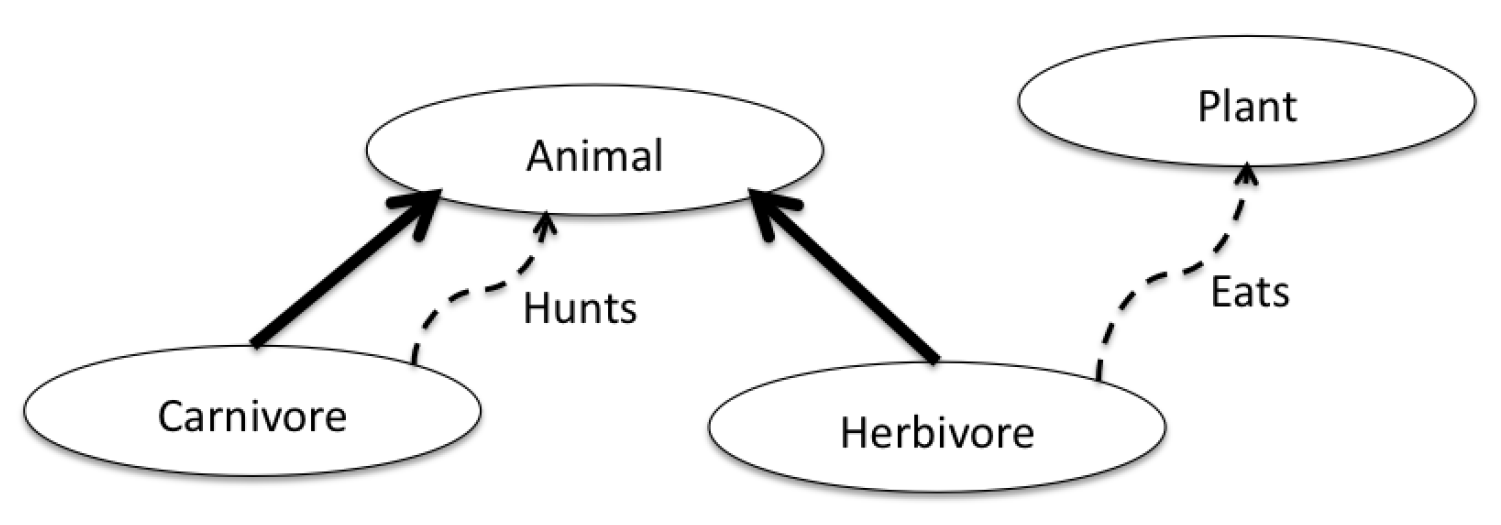
\includegraphics[scale=.33]{img/relationship_network.png}
\caption{An example of network, showing relationships between concepts.}
\label{rel_net}
\end{figure}

Typically, nodes are used to characterize concepts, i.e., sets of individuals, and links are used to characterize relationships among them.
Concepts can have simple properties, which are typically attached to the corresponding nodes.
It is rather simple to make a correspondence between network structures and Description Logics because the latter are equipped with unary predicates representing sets of individuals, binary predicates representing relationships among them, and a mechanism of inclusion statements to express concept properties.

\newpage

Indeed, we can represent concept properties with the inclusion statement $Carnivore \sqsubseteq Animal$, and we can express the following facts about an individual $lion$: 

\begin{itemize}
	\item $Carnivore(lion)$
	\item $Hunts(lion, zebra)$
	\item $Herbivore(elephant)$
	\item $Eats(elephant, grass)$
\end{itemize}

It is also possible to use intersection concepts with the syntax $Carnivore \sqcap Plant$ to select individuals which belong to both $Carnivore$ and $Plant$.


\section{Application domains}
Description Logics are used in the implementation of many systems that demonstrate their practical effectiveness. Some of these systems have found their way into production use, despite the fact that there was no real commercial platform that could be used for developing them.\\

\textbf{Software engineering.} Software Engineering was one of the first application domains for Description Logics. The basic idea was to use a Description Logic to implement a Software Information System, i.e. a system that would support the software developer by helping him in finding out information about a large software system.\\

\textbf{Configuration management.} One very successful domain for knowledge-based applications built using Description Logics is configuration management, which includes applications that support the design of complex systems created by combining multiple components.
The main goal of this discipline is finding a proper set of components that can be suitably connected in order to implement a system that meets a given specification.
For example, choosing computer components in order to build a home PC is a relatively simple configuration task.
When the number, the type, and the connectivity of the components grow, the configuration task can become rather complex.
In particular, computer configuration has been among the application fields of the first Expert Systems and can thus be viewed as a standard application domain for knowledge based systems.

Configuration tasks arise in many industrial domains, such as telecommunications, the automotive industry, building construction, etc.
DL--based knowledge representation systems meet the requirements for the development of configuration applications.
In particular, they enable the object--oriented modelling of system components, which combines powerfully with the ability to reason from incomplete specifications and to automatically detect inconsistencies.
Using Description Logics, one can exploit the ability to classify the components and organize them within a taxonomy.\\

\textbf{Medicine.} Medicine is also a domain where Expert Systems have been developed since the 1980’s, in particular in the field of decision support for medical diagnosis. One focus has been on the construction and maintenance of very large ontologies of medical knowledge, the subject of some large government initiatives.
In order to cope with the scalability of the knowledge base, the DL language adopted in these applications is often limited to a few basic constructs and the knowledge base turns out to be rather shallow, that is to say the taxonomy does not have very many levels of sub--concepts below the top concepts.\\

\textbf{Data mining.} Description Logics have also been used in data mining applications, where their inferences can help the process of analysing large amounts of data.
In this kind of application, DL structures can represent views, and DL systems can be used to store and classify such views. The classification mechanism can help in discovering interesting classes of items in the data
\cite{Nardi:2003:IDL:885746.885748}.

\newpage

\section{Basic Description Logics}
As the name Description Logics indicates, one of the characteristics of these languages is that they are equipped with a formal, logic--based semantics.
Another distinguished feature is the emphasis on reasoning as a central service: reasoning allows one to infer implicitly represented knowledge from the knowledge that is explicitly contained in the knowledge base.\\

Description Logics support inference patterns that occur in many applications of intelligent information processing systems, and which are also used by humans to structure and understand the world: classification of concepts and individuals.

Classification of concepts determines subconcept/superconcept relationships (called subsumption relationships in DL) between the concepts of a given terminology, and thus allows one to structure the terminology in the form of a subsumption hierarchy.

Classification of individuals (or objects) determines whether a given individual is always an instance of a certain concept (i.e., whether this instance relationship is implied by the description of the individual and the definition of the concept). It thus provides useful information on the properties of an individual.
Moreover, instance relationships may trigger the application of rules that insert additional facts into the knowledge base.\\

The implementation of reasoning services requires building procedures that should always terminate, both for positive and for negative answers, but also complexity needs to be taken into consideration.
Decidability and complexity of the inference problems depend on the expressive power of the DL at hand.
On the one hand, very expressive DLs are likely to have inference problems of high complexity.
On the other hand, very weak DLs (with efficient reasoning procedures) may not be sufficiently expressive to represent the important concepts of a given application.

Investigating this trade--off between the expressivity of DLs and the complexity of their reasoning problems is one of the most important issues in DL research
\cite{Baader:2003:BDL:885746.885749}.


\newpage

%%%TODO: DA RIORDINARE
%%% TBox: definire bene, con inclusioni
%%% metti esempio di reasoning, qui o all'inizio
%%% metti bene i modelli mu = <delta^I>

% netta asimmetria tra la descrizione delle DL generali e le logiche con la T
% siccome partiamo dal AL, ..., ci vorrebbero le cose che poi introduciamo dopo:
%	- introduzione, già nelle DL, di quello che facicamo a pagina 9
%		una KB è fatta da TBox e ABox, la TBox contiene le inclusioni, le inclusioni sono fatte così (esempio), ecc <= facciamolo anche prima di entrare nel dettaglio tecnico delle DL classiche
%		*** diciamo come è fatta una TBox (dire che è fatta da inclusioni o da definizioni di ruoli)
%		*** inserire alcuni esempi (di reasoning)- o dopo aver definito AL, o all'inizio, o dopo ALC -
%			^- l'importante è metterlo prima di arrivare a dire cos'è ALC+T
%		*** inserire i modelli (nel caso classico) - non si può dare la definizione dell'interpretazione dei concetti senza sapere cos'è I (metterlo meglio, come c'è nella parte per ALC+T);
%
%

\section{The basic description language $\al$}
A knowledge representation system based on Description Logics provides facilities to set up knowledge bases, to reason about their content, and to manipulate them.

A knowledge base (KB) comprises two components, the TBox and the ABox.

The TBox introduces the terminology, i.e., the vocabulary of an application domain, and contains inclusions or definitions of roles.\\[.2cm]
As an example of TBox, here we have a fraction of a hierarchy of animals. To represent that the penguins are birds and that both the birds and the cats are animals, we have
\begin{center}
$Penguin \sqsubseteq Bird$\\
$Bird \sqsubseteq Animal$\\
$Cat \sqsubseteq Animal$
\end{center}


The ABox contains assertions about named individuals in terms of this vocabulary.\\[.2cm]
For instance, an ABox can contain the following facts
\begin{center}
$Bird(tweety)$\\
$Cat(sylvester)$\\
$Hates(sylvester, tweety)$
\end{center}
representing that Tweety is a bird, Sylvester is a cat, and that Sylvester hates Tweety, respectively.\\[.2cm]
The vocabulary consists of concepts, which denote sets of individuals, and roles, which denote binary relationships between individuals.

Elementary descriptions are atomic concepts and atomic roles.

Complex descriptions can be built from them inductively with concept constructors.\\



In abstract notation, we use the letters $A$ and $B$ for atomic concepts, the letter $R$ for atomic roles, and the letters $C$ and $D$ for concept descriptions.
In the sequel we present the language $\al$ (Attributive concept Language), that has been introduced in \cite{Schmidt-SchaubB:1991:ACD:114341.114342} as a minimal language that is of practical interest. The other languages of this family are extensions of $\al$.

\newpage

\subsection{Syntax}

Concept descriptions in $\al$ are formed according to the following syntax rule:

\begin{itemize}
\item[] $C, D \imp$
\item[] \itab{$A \tc$} \tab{(atomic concept)}
\item[] \itab{$\vero \tc$} \tab{(top concept - most general)}
\item[] \itab{$\falso \tc$} \tab{(bottom concept - most specific)}
\item[] \itab{$\neg A \tc$} \tab{(atomic negation)}
\item[] \itab{$C \mint D \tc$} \tab{(intersection)}
\item[] \itab{$\forall R.C \tc$} \tab{(value restriction)}
\item[] \itab{$\exists R.\vero $} \tab{(limited existential quantification)}
\end{itemize}


\subsection{Semantics}

In order to define a formal semantics of $\al$-concepts we consider interpretations $\II$ that consist of a non--empty set $\Delta$ (the domain of the interpretation) and an interpretation function, which assigns to every atomic concept $A$, a set $A^{\II} \subseteq \Delta^{\II}$ (the set of the individuals of the domain which belong to such concept), and to every atomic role $R$ a binary relation, $R^{\II} \subseteq \Delta^{\II} \times \Delta^{\II}$ (which is a couple of elements of the domain).

\begin{figure}[!htp]
\centering
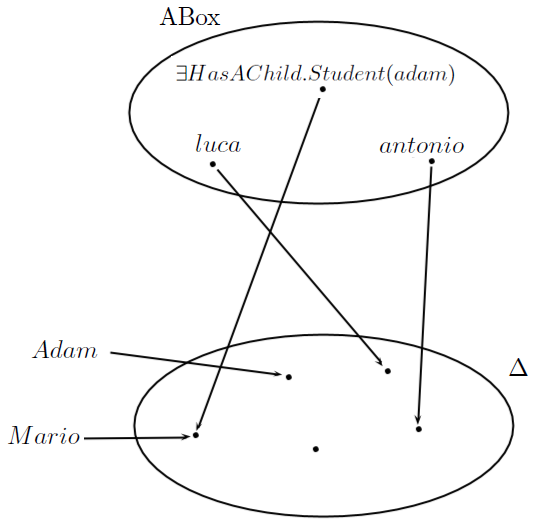
\includegraphics[scale=.50]{img/diagram1_1.png}
\caption{The arrows represent the assignments established by $\II$}
\label{}
\end{figure}


For instance if we have a domain that contains some individuals, some are birds and some are not:
\begin{center}
$Bird \xrightarrow{\mathcal{I}} Bird^{\mathcal{I}}$
\end{center}

The interpretation function is extended to concept descriptions by the following
inductive definitions:

\begin{itemize}
\item[] \itab{$\vero^{\II} = \Delta^{\II}$}
\item[] \itab{$(\neg A)^{\II} = \Delta^{\II} $\textbackslash $A^{\II}$}
\item[] \itab{$(C \mint D)^{\II} = C^{\II} \mint D^{\II}$}
\item[] \itab{$(\forall R.C)^{\II} = \left\{x \in \Delta \tc \perogni y.(x, y)\in R^{\II} \imp y \in C^{\II} \right\}$}
\item[] \itab{$(\exists R.\vero)^{\II} = \left\{x \in \Delta \tc \esiste y.(x, y)\in R^{\II} \right\}$}
\end{itemize}

We say that two concepts $C$, $D$ are equivalent, and write $C = D$, if $C^{\II} = D^{\II}$ for all interpretations $\II$
\cite{Baader:2003:BDL:885746.885749}.\\


A model is a structure $\mathcal{M} = \langle \Delta, \mathcal{I}\rangle$, where:
\begin{itemize}
\item $\Delta$ is the domain;
\item $\mathcal{I}$ is the extension function that maps each extended concept $C$ to $C^\mathcal{I} \subseteq \Delta$, every atomic concept $A \in C$ to a set $C^\mathcal{I} \subseteq \Delta$, and each role $R$ to a $R^\mathcal{I} \subseteq \Delta \times \Delta$.
\end{itemize}

The models attribute a meaning to the inclusions: a certain inclusion $C \sqsubseteq D$ holds in a model $\mathcal{M}$ if $C^\mathcal{I} \sqsubseteq D^\mathcal{I}$.


For instance, the model $\mathcal{M}_{1}$ confirms the inclusion $Penguin \sqsubseteq Bird$ since the extension of the penguins ($Penguin^{\mathcal{I}}$) is included in the extension of the birds ($Bird^{\mathcal{I}}$).

\begin{figure}[H]
\centering
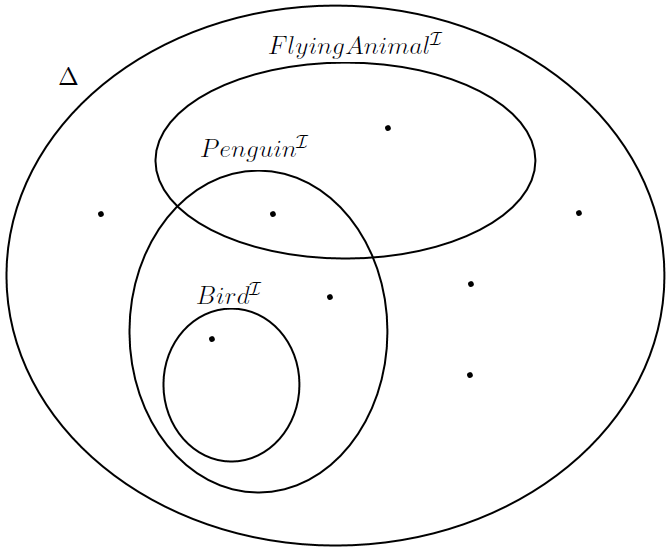
\includegraphics[scale=.34]{img/diagram1_2.png}
\caption{The model $\mathcal{M}_1$}
\label{}
\end{figure}

\vspace{1.0cm}

If we had another model made as $\mathcal{M}_{2}$, in which some of the penguins are not birds, the inclusion would not hold.

\begin{figure}[H]
\centering
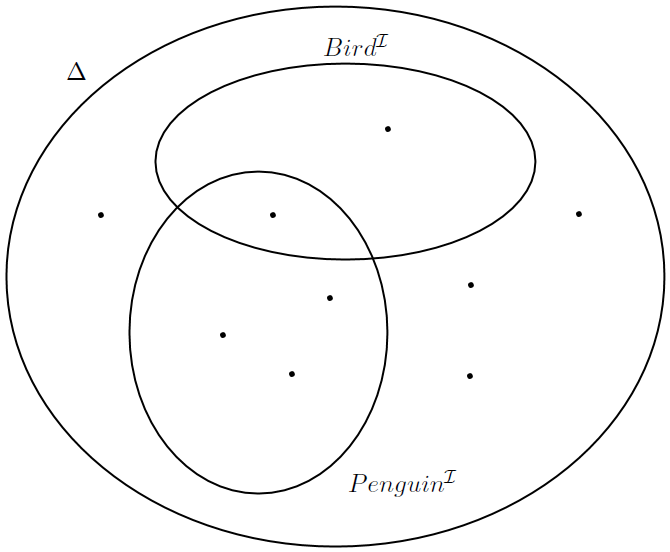
\includegraphics[scale=.34]{img/diagram1_3.png}
\caption{The model $\mathcal{M}_2$}
\label{}
\end{figure}

\section{Complex concept negation: $\alc$}
A basic extension of $\al$ is $\alc$ (Attributive concept Language with Complements), which introduces (see \cite{obitko}) the negation of an arbitrary concept:
\begin{itemize}
\item[] \itab{$\neg C$} \tab{(concept negation)}
\end{itemize}

whose semantics is:
\begin{itemize}
\item[] \itab{$(\neg C)^{\II} = \Delta^{\II} $\textbackslash $C^{\II}$} 
\end{itemize}

This allows us to express notions such as:
\begin{center}
$Penguin \sqsubseteq \neg FlyingAnimal$
\end{center}

Another addition is that in $\alc$ the existential quantification is qualified\footnote{In the traditional $\alc$ we had only $\exists R.\top)$.}, i.e. we admit assertions as

\begin{itemize}
\item[] \itab{$\exists R.C$} \tab{(full quantification)}
\end{itemize}


Its semantics is:
\begin{itemize}
\item[] \itab{$\{a \in \Delta^\mathcal{I}|\exists b.(a, b)\in R^\mathcal{I} \wedge b \in C^\mathcal{I}\}$}
\end{itemize}

\newpage

\section{Non--monotonic reasoning and the operator $\tip$}\label{nonmonotonic_reasoning}
Since the very objective of the TBox is to build a taxonomy of concepts, the need of representing prototypical properties and of reasoning about defeasible inheritance of such properties easily arises.
The traditional approach is to handle defeasible inheritance by integrating some kind of non--monotonic reasoning mechanism.

This has led to study non--monotonic extensions of DLs \cite{baader95a, baader95b, bonattilutzwolterkr06, casinistraccia2010, donini98, donini2002, eiter2004, straccia93}.

However, finding a suitable non--monotonic extension for inheritance reasoning with exceptions is far from obvious.
To give a brief account, \cite{baader95a} proposes the extension of DL with Reiter's default logic.
However, the same authors have pointed out that this integration may lead to both semantical and computational difficulties.

Indeed, the unsatisfactory treatment of open defaults via Skolemization may lead to an undecidable default consequence relation. For this reason, \cite{baader95a} proposes a restricted semantics for open default theories, in which default rules are only applied to individuals explicitly mentioned in the ABox.
Furthermore, Reiter's default logic does not provide a direct way of modeling inheritance with exceptions.
This has motivated the study of extensions of DLs with prioritized defaults
\cite{straccia93,baader95b}.

A more general approach is undertaken in \cite{donini2002}, where it is proposed an extension of DL with two epistemic operators. This extension allows to encode Reiter's default logic as well as to express epistemic concepts and procedural rules.

In \cite{bonattilutz} the authors propose an extension of DL with circumscription. One of the motivating applications of circumscription is indeed to express prototypical properties with exceptions, and this is done by introducing ``abnormality'' predicates, whose extension is minimized.
The authors provide decidability and complexity results based on theoretical analysis.

A tableau calculus for circumscriptive $\mathcal{ALCO}$ is presented in \cite{hitzlertableau}.

In \cite{casinistraccia2010,stracciaijcai2011} a non--monotonic extension of $\mathcal{ALC}$  based on the application of Lehmann and Magidor's \emph{rational closure} \cite{whatdoes} to $\mathcal{ALC}$ is proposed. The approach is based on the introduction of a consequence relation $\ent$ among concepts and of a consequence relation $\Vdash$ among an unfoldable KB and assertions. The authors show that such consequence relations are \emph{rational}. It is also shown that such relations inherit the same computational complexity of the underlying DL.

Recent works discuss the combination of open and closed world reasoning in DLs. In particular, formalisms have been defined for combining DLs with logic programming rules (see, for instance, \cite{eiter2004} and \cite{rosatiacm}). A grounded circumscription approach for DLs with local closed world capabilities has been defined in \cite{hitzlerdl}.\\

Another approach, presented in \cite{tr2008} and expanded in \cite{trfundam} \cite{FI09}, \cite{aiia2011}, \cite{tableaux2011DLs}, \cite{Giordano:2013:NDL:2435476.2435957}, and \cite{conf/aiia/GiordanoGJOP13}, proposes the use of a typicality operator, $\tip$, for extending $\alc$ and allow a form of non--monotonic reasoning in Description Logics.\\

A non--monotonic extension should have the following characteristics:

\begin{enumerate}
\item The (non--monotonic) extension must have a clear semantics and should be based on the same semantics as the underlying monotonic DL;
\item The extension should allow to specify prototypical properties in a natural and direct way;
\item The extension must be decidable, if  so is the underlying monotonic DL, and standard proof methods for monotonic DL should be generalized to it.
\end{enumerate}

Before entering the technical details, let us sketch how the pre--existent work makes use of the typicality operator $\tip$ for inference. The KB is comprised of the standard TBox and ABox, with the addition of a set of assertions of the form $\tip(C)\sqsubseteq D$, where $D$ is a concept not mentioning $\tip$.

For instance, let the TBox contain:

\begin{quote}
$\tip (\mathit{Student}) \sqset \mathit{\neg IncomeTaxPayer}$\\
$\tip (\mathit{Student} \mint \mathit{Worker})  \sqset \mathit{IncomeTaxPayer}$\\
$\tip (\mathit{Student} \mint \mathit{Worker} \mint \mathit{Erasmus})  \sqset \mathit{\neg IncomeTaxPayer}$
\end{quote}


\noindent corresponding to the assertions: typical students don't have to pay income taxes, whereas if a student is also a worker, typically he will pay income taxes; if an Erasmus Programme student is also a worker, he does not have to pay income taxes.
Suppose  further that the ABox contains alternatively one of the following facts:

\begin{quote}
1. $\mathit{Student}(\mathit{luca})$ \\
2. $\mathit{Student}(\mathit{antonio}), \mathit{Worker}(\mathit{antonio})$ \\
3. $\mathit{Student}(\mathit{marco}), \mathit{Worker}(\mathit{marco}), Erasmus(\mathit{marco})$
\end{quote}


\noindent From the different combinations of TBox and one of the above ABox assertions (either $1$ or $2$ or $3$), we can infer the expected (defeasible) conclusions. These are, respectively:

\begin{quote}
1. $\mathit{\neg IncomeTaxPayer}(\mathit{luca})$\\
2. $\mathit{IncomeTaxPayer}(\mathit{antonio})$ \\
3. $\mathit{\neg IncomeTaxPayer}(\mathit{marco})$
\end{quote}

\noindent Moreover, we would also like to infer (defeasible) properties of individuals implicitly introduced by existential restrictions, for instance, if the ABox contains

\begin{quote}
$\exists \mathit{HasChild}.\mathit{Student(grazia)}$
\end{quote}

\noindent we would like to infer that:
\begin{quote}
$\exists \mathit{HasChild.\neg IncomeTaxPayer(grazia)}$
\end{quote}

\noindent Finally, adding irrelevant information should not affect the conclusions. From the TBox above, one should be able to infer as well

\begin{quote}
$\tip (\mathit{Student} \mint \mathit{Tall}) \sqset \mathit{\neg IncomeTaxPayer}$\\
$\tip (\mathit{Student} \mint \mathit{Worker} \mint \mathit{Tall})  \sqset \mathit{IncomeTaxPayer}$ \\
$\tip (\mathit{Student} \mint Worker \mint Erasmus \mint \mathit{Tall})  \sqset \mathit{\neg IncomeTaxPayer}$
\end{quote}

\noindent as  $\mathit{Tall}$ is irrelevant with respect to paying income taxes or not. For the same reason, the conclusion about $\mathit{luca}$ being an instance of $\neg IncomeTaxPayer$ or not should not be influenced by adding $\mathit{Tall}(\mathit{luca})$ to the ABox.\\

Hereinafter we present a non--monotonic extension for defeasible reasoning in description logics, called $\alctmin$, that extends the logic $\alct$ (which introduced the typicality operator \tip).

\newpage

%****************************************************
%******************  DL + T  ************************
%****************************************************

\chapter{Description Logics for typicality}\label{dlt}

\section{The logic $\alct$}\label{alct}


In this section, we recall the original $\alct$, which is an extension of $\alc$ by a typicality operator $\tip$ introduced in \cite{FI09}.

\subsection{Syntax}
Given an alphabet of concept names $\mathcal{C}$, of role names $\mathcal{R}$, and of individual constants $\mathcal{O}$, the language $\elle$ of the logic $\alct$ is defined by distinguishing \emph{concepts} and \emph{extended concepts} as follows:

\begin{itemize}
\item (Concepts)
  \begin{itemize}
     \item $A \in \mathcal{C}$, $\vero$ and $\bot$ are \emph{concepts} of
$\elle$;
    \item if $C, D \in \elle$ and $R \in \mathcal{R}$, then $C
\sqcap D, C \sqcup D, \neg C, \forall R.C, \exists R.C$ are
\emph{concepts} of $\elle$
  \end{itemize}
\item (Extended concepts)
    \begin{itemize}
       \item if $C$ is a
concept of $\elle$, then $C$ and $\tip(C)$ are \emph{extended concepts} of $\elle$
     \item boolean combinations of extended concepts are extended
concepts of $\elle$.
    \end{itemize}
\end{itemize}

\noindent  As in standard $\mathcal{ALC}$, a knowledge base is a pair (TBox, ABox).

The TBox contains subsumptions $C \sqsubseteq D$, where $C \in \elle$ is an extended concept of the form either $C'$ or $\tip(C')$, and $C', D \in \elle$ are concepts.

The ABox contains expressions of the form $C(a)$ and $aRb$ where $C \in \elle$ is an extended concept, $R \in \mathcal{R}$, and $a, b \in \mathcal{O}$.

\newpage

\subsection{Semantics}

In order to provide a semantics to the operator $\tip$, we extend the definition of a model used in ``standard'' terminological logic $\alc$:

\begin{definition}[Semantics of $\tip$ with selection function]\label{Semantics with f_tip} A model is any structure $\langle \Delta, I, f_\tip \rangle$ where:

\begin{itemize}
\item $\Delta$ is the domain, whose elements are denoted with $x, y, z, \dots$;
\item $I$ is the extension function that maps each extended concept $C$ to $C^I \subseteq \Delta$, and each role $R$ to a $R^I \subseteq \Delta \times \Delta$.
$I$ assigns to each atomic concept $A \in \mathcal{C}$ a set $A^I \subseteq \Delta$ and it is extended to arbitrary extended concepts as follows:

\begin{itemize}
  \item $\top^I=\Delta$
  \item $\bot^I=\vuoto$
  \item $(\nott C)^I=\Delta \backslash C^I$
  \item $(C \sqcap D)^I=C^I \cap D^I$
  \item $(C \sqcup D)^I=C^I \cup D^I$
  \item $(\forall R.C)^I=\{x \in \Delta \tc \forall y. (x,y) \in R^I \imp y \in C^I\}$
  \item $(\exists R.C)^I=\{x \in \Delta \tc \exists y.(x,y) \in R^I \ \mbox{and} \ y \in C^I\}$
  \item $(\tip(C))^I = f_\tip(C^I)$
\end{itemize}


\item Given $S \subseteq \Delta$, $f_\tip$ is a function $f_\tip : Pow(\Delta) \rightarrow Pow(\Delta)$ satisfying the following properties:

\begin{itemize}
\item $(f_\tip-1)$ $f_\tip(S) \subseteq S$;
\item $(f_\tip-2)$ if $S \neq \emptyset$, then also $f_\tip(S)
\neq \emptyset$;
\item $(f_\tip-3)$ if $f_\tip(S) \subseteq R$, then $f_\tip(S) = f_\tip(S \cap R)$;
\item $(f_\tip-4)$ $f_\tip(\bigcup S_i ) \subseteq \bigcup f_\tip(S_i)$;
\item $(f_\tip-5)$ $\bigcap f_\tip(S_i) \subseteq  f_\tip(\bigcup S_i)$.
\end{itemize}

\end{itemize}

\end{definition}

\noindent Intuitively, given the extension of some concept $C$, the selection function $f_\tip$ selects  the {\em typical} instances of $C$.

($f_\tip-1$) requests that typical elements of $S$ belong to $S$.

($f_\tip-2$) requests that if there are elements in $S$, then there are also {\em typical} such elements.

The following properties constrain the behaviour of $f_\tip$ with respect to $\cap$ and $\cup$ in such a way that they do not entail monotonicity.

According to ($f_\tip-3$), if the typical elements of $S$ are in $R$, then they coincide with the typical elements of $S \cap R$, thus expressing a weak form of monotonicity (namely, {\em cautious monotonicity}).

($f_\tip-4$) corresponds to one direction of the equivalence $f_\tip(\bigcup S_i) = \bigcup f_\tip(S_i)$, so that it does not entail monotonicity.

Similar considerations apply to the equation $f_\tip(\bigcap S_i) = \bigcap f_\tip(S_i)$, of which only the inclusion $\bigcap f_\tip(S_i) \incluso f_\tip(\bigcap S_i)$ holds.

($f_\tip-5$) is a further constraint on the behavior of $f_\tip$ with respect to arbitrary unions and intersections; it would be derivable if $f_\tip$ were monotonic.

\begin{figure}[H]
\centering
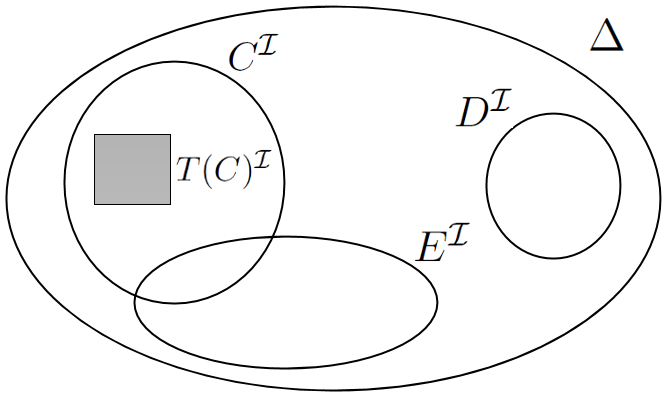
\includegraphics[scale=0.40]{img/diagram1_8.png}
\caption{$f$ selects the typical elements of $C^\mathcal{I}$ (greyed out)}
\label{}
\end{figure}

In \cite{FI09}, it is shown that one can give an equivalent, alternative semantics for $\tip$ based on a \emph{preference relation} semantics rather than on a selection function semantics.

The idea is that there is a global, irreflexive and transitive relation among individuals and that the typical members of a concept $C$ (i.e., those selected by $f_\tip(C^I)$) are the minimal elements of $C$ with respect to this relation.

Observe that this notion is \emph{global}, that is to say, it does not compare individuals with respect to a specific concept.
For this reason,  we cannot express the fact that $y$ is more typical than $x$ with respect to concept $C$, whereas $x$ is more typical than $y$ with respect to another concept $D$.

All we can say is that either $x$ is incomparable with $y$, or $x$ is more typical than $y$, or $y$ is more typical than $x$.
In this framework, an element $x \in \Delta$ is a {\em typical instance} of some concept $C$ if $x \in C^I$ and there is no $C$-element in $\Delta$ {\em more typical} than $x$.\\


The typicality preference relation is partial since it is not always possible to establish given two element which one of the two is more typical.

Following KLM, the preference relation also satisfies a \emph{Smoothness Condition}, which is related to the well known \emph{Limit Assumption} in Conditional Logics \cite{Nute80}
\footnote{More precisely, the Limit Assumption entails the Smoothness Condition (i.e. that there are no infinite $<$ descending chains). Both properties come for free in finite models.};
this condition ensures that, if the extension $C^I$ of a concept $C$ is not empty, then there is at least one \emph{minimal} element of $C^I$.

\newpage

This is stated in a rigorous manner in the following definition:

\begin{definition}\label{Definition of $<$} Given an irreflexive and transitive relation  $<$ over a domain $\Delta$, called \emph{preference relation}, for all $S \subseteq \Delta$, we define

\begin{center}$Min_<(S)= \{x \in S \tc \nexists y \in S \ \mbox{s.t.} \ y < x \}$\end{center}

\noindent We say that $<$ satisfies the {\em Smoothness Condition} if for all $S \subseteq \Delta$, for all $x \in S$, either $x \in Min_<(S)$ or $\exists y \in  Min_<(S)$ such that $y < x$.
\end{definition}

%%TODO: mettere un disegnino, col modello, C minimali,...
%% ad es: 2 disegni, con 3 individui, far vedere che la funzione seleziona questo e quest'altro, ma allora quello è C minimale, quindi tipico C incluso in D - vedere esempi incontri + caso classico studenti:
%	antonio, mario >> in base alla relazione, mario è un po' più strano, quindi antonio gli è preferito
%	gli studenti minimali non pagano le tasse (perchè sono studenti tipici), antonio  (perchè è uno studente lavoratore, quindi non tipico) paga le tasse   <<<<=== nei 2 casi far vedere i due tipi di modelli

\begin{figure}[h]
\centering
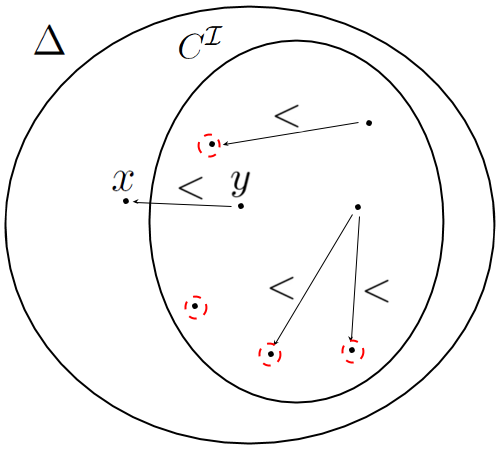
\includegraphics[scale=.40]{img/diagram1_9.png}
\caption{The typical individuals of $C$ (i.e. the individuals which are $\tip(C)$) are highlighted in the figure. $x$ is preferred to $y$, but it is not a $\tip(C)$ since it is not in $C^{\mathcal{I}}.$}
\label{rel_preferenza}
\end{figure}


\noindent The following representation theorem is proved in \cite{FI09}:

\begin{theorem}[Theorem 2.1 in \cite{FI09}]\label{rtrt} Given any model $\langle \Delta, I, f_\tip
\rangle$, $f_\tip$ satisfies postulates $(f_\tip-1)$ to $(f_\tip-5)$ above iff there exists  an irreflexive and transitive relation $<$ on $\Delta$, satisfying the Smoothness Condition, such that for all $S \subseteq \Delta$, $f_\tip(S) = Min_<(S)$.
\end{theorem}

\newpage

\noindent Having the above Representation Theorem, from now on, we will refer to the following semantics:

\begin{definition}[Semantics of $\alct$]\label{Semantics of T} A model $\emme$ of $\alct$ is any structure $$\langle \Delta, I, < \rangle$$ where:

\begin{itemize}

\item $\Delta$ is the domain;

\item $<$ is an irreflexive and transitive relation over $\Delta$ satisfying the Smoothness Condition (Definition \ref{Definition of $<$})

\item $I$ is the extension function that maps each  extended concept $C$ to $C^I \subseteq \Delta$, and each role $R$ to a $R^I \subseteq \Delta \times \Delta$.
$I$ assigns to each atomic concept $A \in \mathcal{C}$ a set $A^I \subseteq \Delta$.
Furthermore, $I$ is extended as in Definition \ref{Semantics with f_tip} with the exception of $(\tip(C))^I$, which is defined as $$(\tip(C))^I = Min_<(C^I).$$
\end{itemize}

\end{definition}

\subsection{Satisfiability}

\noindent Let us now introduce the notion of satisfiability of an $\alct$ knowledge base.

In order to define the semantics of the assertions of the ABox, we  extend the function $I$ to individual constants;  we assign to each individual constant $a \in \mathcal{O}$ a \emph{distinct} domain element $a^I \in \Delta$, that is to say we enforce the \emph{unique name assumption}, i.e. distinct domain elements are associated to different constant names in the ABox.

As usual, the adoption of the  unique name assumption greatly simplifies reasoning about prototypical properties of individuals denoted by different individual constants.\\

%%%TODO: mettere anche qui il disegnino con i Min_<(C^I)

Considering the example of students and taxpayers, if (in addition to the TBox) the ABox only contains the following facts about Luca and Antonio:

\begin{quote}
$\mathit{Student}(\mathit{luca})$ \\
$\mathit{Student}(\mathit{antonio}), \mathit{Worker}(\mathit{antonio})$
\end{quote}

\noindent we would like to infer that Antonio pays the taxes, whereas Luca does not; but without the unique name hypothesis, we cannot draw this conclusion since Luca and Antonio might be the same individual.\\

To perform useful reasoning we would need to  extend the language with equality and make a case analysis according to possible identities of individuals. While this is technically possible, we prefer to keep the things simple here by adopting the unique name assumption.

\begin{definition}[Model satisfying a Knowledge Base]\label{Def-ModelSatTBox-ABox} Consider a model $\emme$, as defined in Definition \ref{Semantics of T}.
We extend $I$ so that it assigns to each individual constant $a$ of $\mathcal{O}$ an element $a^I \in \Delta$,  and $I$ satisfies the unique name assumption. Given a KB (TBox,ABox), we say that:

\begin{itemize}
\item $\emme$  satisfies TBox iff  for all  inclusions $C \sqsubseteq D$  in TBox, $C^I \subseteq D^I$.
\item $\emme$ satisfies ABox  iff:
(i) for all $C(a)$  in ABox, we have that $a^I \in C^I$,
(ii) for all $aRb$ in ABox, we have that $(a^I,b^I) \in R^I$.
\end{itemize}

\noindent $\emme$ satisfies a knowledge base if it satisfies both its TBox and its ABox.

Last, a query $F$  is  entailed by KB in $\alct$ if it holds in all models satisfying \emph{KB}.

In this case we write \emph{KB} $\models_{\alct} F$.\\
\end{definition}


\noindent Notice that the meaning of $\tip$ can be split into two parts.

For any $x$ of the domain $\Delta$,  $x \in (\tip(C))^I$ just in case:
\begin{enumerate}
\item $x \in C^I$;
\item there is no $y \in C^I$ such that $y < x$.
\end{enumerate}
As already mentioned in the Introduction, in order to isolate the second part of the meaning of $\tip$ (for the purpose of the calculus that we will present in Section \ref{tab}), we introduce a new modality, $\bbox$.\\

The basic idea is simply to interpret the preference relation $<$ as an accessibility relation.
By the Smoothness Condition, it turns out that $\bbox$ has the properties as in G\"odel-L\"ob modal logic of provability G.

The Smoothness Condition ensures that typical elements of $C^I$ exist whenever $C^I \diverso \vuoto$, by avoiding infinitely descending chains of elements.
This condition therefore corresponds to the finite-chain condition on the accessibility relation (as in G).\\

The interpretation of $\bbox$ in $\emme$ is as follows:

\begin{definition}\label{def-box}
Given a model $\emme$ as in Definition \ref{Semantics of T}, we extend the definition of $I$ with the following clause:
\begin{center}
	$(\bbox C)^I = \{x \in \Delta \tc $  for every $y \appartiene \Delta$, if $y < x$ then $y \in C^I \}$
\end{center}
\end{definition}

\newpage

\noindent It is easy to observe that $x$ is a typical instance  of $C$ if and only if it is an instance of $C$ and $\bbox \nott C$, that is to say:

\begin{proposition}\label{Relation between T an box}
Given a model $\emme$ as in Definition \ref{Semantics of T}, given a concept $C$ and an element $x \in \Delta$, we have that $$x \in (\tip(C))^I \ \mbox{iff} \  x \in (C \sqcap \bbox \neg C)^I$$
\end{proposition}

\noindent
Since we only use $\bbox$ to capture the meaning of $\tip$, in the following we will always use the modality $\bbox$ followed by a negated concept, as in $\bbox \neg C$.

The Smoothness condition, together with the transitivity of $<$, ensures the following Lemma:

\begin{lemma}\label{ssc}
Given an $\alct$ model as in Definition \ref{Semantics of T}, an extended concept $C$, and an element $x \in \Delta$, if there exists $y < x$ such that $y \in C^I$, then either $y \in Min_<(C^I)$ or there is $z<x$ such that $z \in Min_<(C^I)$.
\end{lemma}

\begin{proof}
See \cite{Giordano:2013:NDL:2435476.2435957}.
\end{proof}


Last, we state a theorem which will be used in the following:

\begin{theorem}[Finite model property of $\alct$]\label{fmpALCT}
The logic $\alct$ has the finite model property.
\end{theorem}

\begin{proof}
See \cite{Giordano:2013:NDL:2435476.2435957}.
\end{proof}

\newpage

\section{The logic $\alctmin$}\label{alctmin}

As mentioned in the Introduction, the logic $\alct$ presented in \cite{FI09} allows  to reason about typicality.
As a difference with respect to standard $\alc$, in $\alct$ we can consistently express, for instance, the fact that three different concepts, like {\em Department member}, {\em Temporary Department Member} and {\em Temporary Department member having restaurant tickets}, have a different status with respect to {\em Have lunch at a restaurant}.

This can be consistently expressed by including in a knowledge base the three formulas:

\begin{quote}
$\tip (\mathit{DepartmentMember}) \sqset \mathit{LunchAtRestaurant}$\\
$\tip (\mathit{DepartmentMember} \mint \mathit{TemporaryResearcher})  \sqset \nott \mathit{LunchAtRestaurant}$\\
$\tip (\mathit{DepartmentMember} \mint \mathit{TemporaryResearcher} \mint \exists \mathit{Owns}.\mathit{RestaurantTicket}) \sqset \mathit{LunchAtRestaurant}$
\end{quote}

\noindent Let us assume that $\mathit{greg}$ is an instance of the concept
\begin{center}$\mathit{DepartmentMember} \sqcap \mathit{TemporaryResearcher} \sqcap \exists \mathit{Owns}.\mathit{RestaurantTicket}$. \end{center}
What can we conclude about $\mathit{\mathit{greg}}$? We have already mentioned that if the ABox explicitly points out that $\mathit{greg}$ is a {\em typical} instance of the  concept, and it contains the assertion that:

\begin{center}$(*)  \ \tip(\mathit{DepartmentMember} \sqcap \mathit{TemporaryResearcher} \sqcap \exists \mathit{Owns}.\mathit{RestaurantTicket})(\mathit{greg}),$\end{center}

%%%TODO: reindentare con più respiro

\noindent then, in $\alct$, we can conclude that

\begin{center}$\mathit{LunchAtRestaurant(\mathit{greg})}.$\end{center}

\noindent However, if (*) is replaced by the weaker
\begin{center} $(**)  \ (\mathit{DepartmentMember} \sqcap \mathit{TemporaryResearcher} \sqcap \exists \mathit{Owns}.\mathit{RestaurantTicket})(\mathit{greg}),$ \end{center}

in which there is no information about the typicality of $\mathit{greg}$, in $\alct$ we can no longer draw this conclusion, and indeed we cannot make any inference about whether $\mathit{greg}$ spends its lunch time at a restaurant or not.\\

The limitation here lies in the fact that $\alct$ is {\em monotonic}, whereas we would like to make a non--monotonic inference.
Indeed, we would like to non--monotonically assume, in the absence of information to the contrary, that $\mathit{greg}$ is a typical instance of the concept.
In general, we would like to infer that individuals are typical instances of the concepts they belong to, if this is consistent with the KB.\\

As a difference with respect to $\alct$, $\alctmin$ is {\em non--monotonic}, and it allows to make this kind of inference.
Indeed, in $\alctmin$ if (**) is all the information about $\mathit{greg}$ present in the ABox, we can derive that $\mathit{greg}$ is a typical instance of the concept, and from the inclusions above we conclude that $\mathit{LunchAtRestaurant(\mathit{greg})}.$\\

We have already mentioned that we obtain this non--monotonic behaviour by restricting our attention to the  minimal $\alct$ models.
As a difference with respect to $\alct$, in order to determine what is entailed by a given knowledge base KB, we do not consider {\em all} models of KB but only the {\em minimal} ones.
These are the models that minimize the number of atypical instances of concepts.\\

Given a KB, we consider a finite set $\ellet$ of concepts occurring in the KB: these are the concepts for which we want to minimize the atypical instances.

The minimization of the set of atypical instances will apply to individuals explicitly occurring in the ABox as well as to implicit individuals.

We assume that the set $\ellet$ contains at least all concepts $C$ such that $\tip(C)$ occurs in the KB.
Notice that in case $\ellet$ contains more concepts than those occurring in the scope of $\tip$ in KB, the atypical instances of these concepts will be minimized but no extra properties will be inferred for the typical instances of the concepts, since the KB does not say anything about these instances.

We have seen that $(\tip(C))^I =(C \sqcap \bbox \neg C)^I$: $x$ is a typical instance  of a concept $C$ ($x \in (\tip(C))^I$) when it is an instance of $C$  and there is no other instance of $C$ preferred to $x$, i.e. $x \in (C \sqcap \bbox \neg C)^I$.

By contraposition an instance of $C$ is atypical if $x \in (\neg \bbox \neg C)^I$ therefore in order to minimize the atypical instances of $C$, we minimize the instances of $\neg \bbox \neg C$.

Notice that this is different from maximizing the instances of $\tip(C)$.
We have adopted this solution since it allows to maximize the set of typical instances of $C$ without affecting the extension $C^I$ of $C$ (whereas maximizing the extension of $\tip(C)$  would imply maximizing also the extension of $C$).\\

We define the set $\emme^{\bbox^-}_{\ellet}$ of negated boxed formulas holding in a model, relative to the concepts in $\ellet$:

\begin{definition}
Given a model $\emme=\sx \Delta, I, <\dx$ and a set of concepts $\ellet$, we define $$\emme^{\bbox^-}_{\ellet}=\{(x, \nott \bbox \nott C) \tc x \in (\nott \bbox \nott C)^I, \ \mbox{with} \ x \in \Delta, C \in \ellet \}$$
\end{definition}

\newpage

\noindent Let KB be a knowledge base and let ${\ellet}$ be a set of concepts occurring in KB.

\begin{definition}[Preferred and minimal models]\label{def preferred and minimal models}
Given a model $\emme=\sx \Delta_{\emme}, I_{\emme}, <_{\emme} \dx$ of KB and  a model $\enne=\sx \Delta_{\enne}, I_{\enne}, <_{\enne} \dx$ of KB, we say that $\emme$ is preferred to $\enne$ with respect to ${\ellet}$, and we write $\emme <_{\ellet} \enne$, if the following conditions hold:

\begin{itemize}
\item $\Delta_{\emme}=\Delta_{\enne}$
\item $a^{I_{\emme}}=a^{I_{\enne}}$ for all individual constants $a \in \begin{mathcal}O\end{mathcal}$
\item $\emme^{\bbox^-}_{\ellet} \subset \enne^{\bbox^-}_{\ellet}$.
\end{itemize}

\noindent A model $\emme$ is a \emph{minimal model} for KB (with respect to ${\ellet}$) if it is a model of KB and there is no a model $\emme'$ of KB such that $\emme' <_{\ellet} \emme$.\\
\end{definition}

\noindent Given the notion of preferred and minimal models above, we introduce a notion of \emph{minimal entailment}, that is to say we restrict our consideration to minimal models only.
First of all, we introduce the notion of \emph{query}, which can be minimally entailed from a given KB.
A query $F$ is  a formula of the form $C(a)$ where $C$ is an extended concept and $a \in \mathcal{O}$.
We assume that, for all $\tip(C')$ occurring in $F$, $C' \in \ellet$.
Given a KB and a model $\emme=\sx \Delta, I, < \dx$ satisfying it, we say that a query $C(a)$ holds in $\emme$ if $a^I \in C^I$.\\

Let us now define minimal entailment of a query in $\alctmin$.

\begin{definition}[Minimal Entailment in $\alctmin$]\label{LogicalConsequenceALCTMIN}
A query $F$  is minimally entailed from a knowledge base \emph{KB} with respect to ${\ellet}$ if it holds in all models of \emph{KB} that are minimal with respect to ${\ellet}$.
We write \emph{KB} $\models_{min}^{\ellet} F$.
\end{definition}


\noindent The non--monotonic character of $\alctmin$ also allows to deal with the following examples.

\vspace{0.5cm}


\noindent {\em Example 1}.
Consider the following KB
\begin{center}
$\tip(\mathit{Athlete}) \sqset \mathit{Confident}$\\
$\mathit{Athlete}(\mathit{john})$\\
$\mathit{Finnish}(\mathit{john})$
\end{center}
and ${\ellet}=
\{\mathit{Athlete}, \mathit{Finnish}\}$.

We have $$\mbox{KB} \
\models_{min}^{\ellet} \mathit{Confident}(\mathit{john})$$

Indeed, there is no minimal model of KB that contains a non--typical instance of some concept (indeed in all minimal models of KB the relation $<$ is empty).

Hence $\mathit{john}$ is an instance of $\tip(\mathit{Athlete})$ (it can be easily verified that any model in which $\mathit{john}$ is not an instance of $\tip(\mathit{Athlete})$ is not minimal).

By KB, in all these models, $\mathit{john}$ is an instance of $\mathit{Confident}$.
Observe that $\mathit{Confident}(\mathit{john})$ is obtained, in spite of the presence of the irrelevant assertion $\mathit{Finnish}(\mathit{john})$.


\vspace{0.35cm}

\noindent {\em Example 2}. Consider now the knowledge base KB' obtained by adding to KB the formula

\begin{center}$\tip(\mathit{Athlete} \mint \mathit{Finnish}) \sqsubseteq \neg \mathit{Confident}$\end{center}

that is to say $KB'$ is 
\begin{center}
$\tip(\mathit{Athlete}) \sqset \mathit{Confident}$\\
$\tip(\mathit{Athlete} \ \mint \ \mathit{Finnish}) \sqsubseteq \neg \mathit{Confident}$\\
$\mathit{Athlete}(\mathit{john})$\\
$\mathit{Finnish}(\mathit{john})$
\end{center}
and let us add to ${\ellet}$ the concept

\begin{center}$\mathit{Athlete} \mint \mathit{Finnish}$\end{center}

From KB', $\mathit{Confident}(\mathit{john})$ is no longer derivable.
Instead, we have that
\begin{center}$\mbox{KB}' \models_{min}^{\ellet} \neg \mathit{Confident}(\mathit{john})$\end{center}

Indeed, by reasoning as above, it can be shown that in all the minimal models of KB', $\mathit{john}$ is an instance of $\tip(\mathit{Athlete} \mint \mathit{Finnish})$, and it is no longer an instance of $\tip(\mathit{Athlete})$.\\

This example shows that, in case of conflict (here, $\mathit{john}$ cannot be both a typical instance of $\mathit{Athlete}$ and of $\mathit{Athlete} \mint \mathit{Finnish}$), typicality in the more specific concept is preferred.

%%%TODO: reindentare con più respiro
% Scrivere la KB con le varie inclusioni messe per disteso

\vspace{0.35cm}

\noindent In general, a knowledge base KB may have no minimal model or more than one minimal model, with respect to a given $\ellet$.\\

The following property holds.

\begin{proposition}\label{proprModMinimali1}
If \emph{KB} has a model, then \emph{KB} has a minimal model with respect to any $\ellet$.
\end{proposition}

The above fact is a consequence of the \emph{finite model property} of the logic $\alct$ (as stated in Theorem \ref{fmpALCT}).


%****************************************************
%*************  TABLEAUX CALCULUS   *****************
%****************************************************


\chapter{A tableaux calculus for $\alctmin$}\label{tab}

In this chapter we present a tableau calculus for deciding whether a query $F$ is minimally entailed by a knowledge base $KB=(TBox,ABox)$.

This calculus, called $\nuovoc$, extends the calculus $\calcolo$ presented in \cite{FI09}, and allows to reason about minimal models.

$\nuovoc$ performs a two--phase computation in order to check whether a query $F$ is minimally entailed from the initial $KB$.
In particular, the procedure tries to build an open branch representing a minimal model satisfying $KB \unione \ \{\nott F\}$.\\

\noindent In the first phase, a tableau calculus, called $\primo$, simply verifies whether $KB \unione \ \{\nott F\}$ is satisfiable in an $\alct$ model, building candidate models.

In the second phase another tableau calculus, called $\secondo$, checks whether the candidate models found in the first phase are \emph{minimal} models of $KB$.

To this purpose, for each open branch of the first phase, $\secondo$ tries to build a ``smaller'' model of $KB$, i.e. a model whose individuals satisfy less formulas $\nott \bbox \nott C$ than the corresponding candidate model. The whole procedure $\nuovoc$ is formally defined at the end of this section (Definition \ref{def processo}).\\

$\nuovoc$ is based on the notion of a \emph{constraint system}.

We consider a set of \emph{variables} drawn from a denumerable set $\mathcal{V}$.

Variables are used to represent individuals not explicitly mentioned in the ABox, that is to say implicitly expressed by existential as well as universal restrictions.\\

$\nuovoc$ makes use of labels, which are denoted with $x, y, z, \dots$.
A label represents either a variable or an individual constant occurring in the ABox, that is to say an element of $\mathcal{O} \unione \mathcal{V}$.

\newpage

\begin{definition}[Constraint]
A \emph{constraint} (or \emph{labelled} formula) is a syntactic entity of the form either $x \trans{R} y$ or $y<x$ or $x: C$, where $x, y$ are labels, $R$ is a role and $C$ is either an extended concept or has the form $\bbox \nott D$ or $\nott \bbox \nott D$, where $D$ is a concept.
\end{definition}

\noindent Intuitively, a constraint of the form $x \trans{R} y$ says that the individual represented by label $x$ is related to the one denoted by $y$ by means of role $R$; a constraint $y<x$ says that the individual denoted by $y$ is ``preferred'' to the individual represented by $x$ with respect to the relation $<$; a constraint $x: C$ says that the individual denoted by $x$ is an instance of the concept $C$, i.e. it belongs to the extension $C^I$.\\

As we will define in Definition \ref{corresponding constraint system}, the ABox of a knowledge base can be translated into a set of constraints by replacing every membership assertion $C(a)$ with the constraint $a: C$ and every role $a R b$ with the constraint $a \trans{R} b$.\\

Let us now separately analyse the two components of the calculus $\nuovoc$, starting with $\primo$.

\section{The tableau calculus $\primo$}\label{tableau_ph1}

Let us first define the basic notions of a tableau system in $\primo$:


\begin{definition}[Tableau of $\primo$]\label{deftableau}
A tableau of $\primo$ is a tree whose nodes are constraint systems, i.e., pairs $\sx S \tc U \dx$, where $S$ is a set of constraints, whereas $U$ contains formulas of the form $C \sqsubseteq D^L$, representing subsumption relations $C \sqsubseteq D$ of the TBox. $L$ is a list of labels
\footnote{As we will discuss later, this list is used in order to ensure the termination of the tableau calculus.}.

A branch is a sequence of nodes $\sx S_1 \tc U_1 \dx, \sx S_2 \tc U_2 \dx, \dots, \sx S_n  \tc U_n \dx \dots$, where each node $\sx S_i \tc U_i \dx$ is obtained from its immediate predecessor $\sx S_{i-1} \tc U_{i-1} \dx$ by applying a rule of $\primo$ (see Figure \ref{immagine calcolo}), having $\sx S_{i-1} \tc U_{i-1} \dx$ as the premise and $\sx S_{i} \tc U_{i} \dx$ as one of its conclusions.

A branch is closed if one of its nodes is an instance of \emph{clash} (either (Clash) or $(\mbox{Clash})_\top$ or $(\mbox{Clash})_\bot$), otherwise it is open. A tableau is closed if all its branches are closed.
\end{definition}

\noindent In order to check the satisfiability of a $KB$, we build the corresponding constraint system $\sx S \tc U \dx$, and we check its satisfiability.

\begin{definition}[Corresponding constraint system]\label{corresponding constraint system}
Given a knowledge base \emph{KB}=$($TBox,ABox$)$, we define its \emph{corresponding constraint system} $\sx S \tc U \dx$ as follows:

\begin{itemize}
 \item $S=\{a: C \tc C(a) \in \mbox{ABox}\} \unione \{a \trans{R} b \tc a R b \in \mbox{ABox}\}$
 \item $U=\{C \sqsubseteq D^{\vuoto} \tc C \sqsubseteq D \in \mbox{TBox}\}$
\end{itemize}

\end{definition}

\begin{definition}[Model satisfying a constraint system]\label{modello constraint}
Let $\emme=\sx \Delta, I, < \dx$ be a model as defined in Definition \ref{Semantics of T}.

We define a function $\alpha$ which assigns to each variable of $\mathcal{V}$ an element of $\Delta$, and assigns every individual constant $a \in \mathcal{O}$ to $a^{I} \in \Delta$.

$\emme$ satisfies  a constraint $F$ under $\alpha$, written $\emme \models_\alpha F$, as follows:

\begin{itemize}
 \item $\emme \models_\alpha x: C$  if and only if $\alpha(x) \in C^{I}$
 \item $\emme \models_\alpha x \trans{R} y$ if and only if $(\alpha(x),\alpha(y)) \in R^{I}$
 \item $\emme \models_\alpha y < x$ if and only if $\alpha(y) < \alpha(x)$
\end{itemize}

A constraint system $\sx S \tc U \dx$ is satisfiable if there is a model $\emme$ and a function $\alpha$ such that $\emme$ satisfies  every constraint in $S$ under $\alpha$ and that, for all $C \sqsubseteq D^L \in U$ and for all $x \in \Delta$, we have that if $x \in C^I$ then $x \in D^I$.
\end{definition}

Let us now show that:

\begin{proposition}\label{corresp constr system} KB=(TBox,ABox) is satisfiable in an $\alct$ model if
and only if its corresponding constraint system $\sx S \tc U \dx$ is satisfiable in the same model.
\end{proposition}

\begin{proof}
See \cite{Giordano:2013:NDL:2435476.2435957}.
\end{proof}


\noindent To verify the satisfiability of $KB \unione \ \{ \nott F\}$, we use $\primo$ to check the satisfiability of the constraint system $\sx S \tc U \dx$ obtained by adding the constraint corresponding to $\nott F$ to $S'$, where $\sx S' \tc U \dx$ is the corresponding constraint system of $KB$.

To this purpose, the rules of the calculus $\primo$ are applied until either a contradiction is generated (\emph{clash}) or a model satisfying $\sx S \tc U \dx$ can be obtained from the resulting constraint system.

As in the calculus proposed in \cite{FI09}, given a node $\sx S \tc U \dx$, for each subsumption $C \sqsubseteq D^L \in U$ and for each label $x$ that appears in the tableau, we add to $S$ the constraint $x: \nott C \unioneq D$: we refer to this mechanism as \emph{subsumption expansion}.

As mentioned above, each subsumption $C \sqsubseteq D$ is equipped with a list $L$ of labels in which the subsumption has been expanded in the current branch.

This is needed to avoid multiple expansions of the same subsumption by using the same label, generating infinite branches.\\


Before introducing the rules of $\primo$ we need some more definitions.

First, as in \cite{buchheit-et-al}, we define an ordering relation $\prec$ to keep track of the temporal ordering of insertion of labels in the tableau, that is to say if $y$ is introduced in the tableau, then $x \prec y$ for all labels $x$ that are already in the tableau.

Moreover, we need to define the \emph{equivalence} between two labels: intuitively, two labels $x$ and $y$ are equivalent if they label the same set of extended concepts.

This notion is stated in the following definition, and it is used in order to apply the blocking machinery described in the following, based on the fact that equivalent labels represent the same element in the model built by $\primo$.

\begin{definition}
Given a tableau node $\sx S \tc U \dx$ and a label $x$, we define
\begin{center}$\sigma(\sx S \tc U \dx,x)=\{C \tc x: C \in S\}.$\end{center}

\noindent Furthermore, we say that two labels $x$ and $y$ are $S$-\emph{equivalent}, written $x \equiv_S y$, if they label the same set of concepts, i.e.

\begin{center}$\sigma(\sx S \tc U \dx,x)=\sigma(\sx S \tc U \dx,y).$\end{center}
\end{definition}

\noindent Last, we define the set of formulas $\Gammam{x}{y}$, that will be used in the rule $(\bbox^-)$ when $y<x$, in order to introduce $y: \nott C$ and $y: \bbox \nott C$ for each $x: \bbox \nott C$ in the current branch:

\begin{definition}
Given a tableau node $\sx S \tc U \dx$ and two labels $x$ and $y$, we define

$$\Gammam{x}{y}=\{y: \nott C, y: \bbox \nott C \tc x: \bbox \nott C \in S\}.$$
\end{definition}

\newpage

\subsection{Rules}

\noindent The rules of $\primo$ are presented in Figure \ref{immagine calcolo}.

\begin{figure}[H]{
\centerline{
	\includegraphics[angle=0,width=14cm]{primoOK}
	}
}
\caption{The calculus $\primo$. To save space, we omit the rules $(\perogni^-)$ and $(\esiste^-)$, dual to $(\esiste^+)$ and $(\perogni^+)$, respectively.}
\label{immagine calcolo}
\end{figure}

The rules $(\esiste^{+})$ and $(\bbox^{-})$ are called \emph{dynamic}, since they introduce a new variable in their conclusions.
The other rules are called \emph{static}.


A brief explanation of the rules follows:

\begin{itemize}
  \item $(\mbox{Clash})$, $(\mbox{Clash})_\top$ and $(\mbox{Clash})_\bot$ are used to detect \emph{clashes}, i.e. unsatisfiable constraint systems;
  
  \item the rules for $\sqcup$, $\sqcap$, $\nott$, and $\forall$ are similar to the corresponding ones in the tableau calculus for standard $\alc$ \cite{buchheit-et-al}: as an example, the rule $(\sqcup^+)$ is applied to a constraint system of the form $\sx S, x: C \sqcup D \tc U \dx$ in order to deal with the constraint $x: C \sqcup D$ introducing two branches in the tableau construction, to check the two conclusions obtained by adding the constraints $x: C$ and $x: D$, respectively. 
  
  The side conditions of the rules are the usual conditions needed to avoid multiple applications on the same principal formula: concerning the example of $(\sqcup^+)$, it can be applied only if $x: C \not \in S$ and $x: D \not\in S$;
  
  \item the rules $(\tip^+)$ and $(\tip^-)$ are used to ``translate'' formulas of the form $\tip(C)$ in the corresponding modal interpretation: for $(\tip^+)$, this corresponds to introduce $x: C \sqcap \bbox \nott C$ to a constraint system containing $x: \tip(C)$, whereas for $(\tip^-)$ a branching is introduced to add either $x: \nott C$ or $x: \nott \bbox \nott C$ in case $x: \nott \tip(C)$ belongs to the constraint system;
  
  \item the rule $(\sqsubseteq)$ is used in order to check whether, for all $x$ belonging to a branch, the inclusion relations of the TBox are satisfied: given a label $x$ and an inclusion $C \sqsubseteq D^L \in U$, the branching introduced by the rule ensures that either $x: \nott C$ holds or that $x: D$ holds;
  
  \item the rule $(\bbox^-)$, applied to a principal formula $x: \nott \bbox \nott C$ ($x$ is not a typical instance of the concept $C$, i.e. there exists an element $z$ which is a typical instance of $C$ and is more normal than $x$), introduces the constraints $z < x$, $z: C$ and $z: \bbox \nott C$.
  
A branching on the choice of the label $z$ to use is introduced, since it can be either a ``new'' label $y$, not occurring in the branch, or one of the labels $v_1, v_2, \dots, v_n$ already belonging to the branch.
We do not need any extra rule for the positive occurrences of the $\bbox$ operator, since these are taken into account by the computation of $\Gammam{x}{y}$ of $(\bbox^-)$. $(\esiste^{+})$ deals with constraints of the form $x: \esiste R.C$ in a similar way.

The additional side conditions on $(\esiste^{+})$ and $(\bbox^{-})$ are introduced in order to ensure a terminating proof search, by implementing the standard \emph{blocking} technique described below.\\
Intuitively, they are applied to constraints $x: \esiste R.C$ and $x: \nott \bbox \nott C$, respectively, only if $x$ \emph{is not blocked}, i.e. if there is no label (\emph{witness}) $z$, labelling the same concepts of $x$, such that the rule has been already applied to $z: \esiste R.C$ (resp. $z: \nott \bbox \nott C$).\\
This is formally stated in Definition \ref{witness} below;

\item the $(cut)$ rule ensures that, given any concept $C \in \ellet$, an open branch built by $\primo$ contains either $x: \bbox \nott C$ or $x: \nott \bbox \nott C$ for each label $x$: this is needed in order to allow $\secondo$ to check the minimality of the model corresponding to the open branch, as we will discuss later.
\end{itemize}


\noindent All the rules of the calculus copy their principal formulas, i.e. the formulas to which the rules are applied, in all their conclusions.
As we will discuss later, for the rules $(\esiste^+)$, $(\perogni^-)$ and $(\bbox^-)$ this is used in order to apply the blocking technique, whereas for the rules $(\esiste^-)$, $(\perogni^+)$, $(\sqsubseteq)$, and $(cut)$ this is needed in order to have a complete calculus.

Rules for $\sqcap$, $\sqcup$, $\nott$, and $\tip$ also copy their principal formulas in their conclusions for uniformity's sake.

\newpage

In order to ensure the completeness of the calculus, the rules of $\primo$ are applied with the following \emph{standard strategy}:
\begin{enumerate}
\item apply a rule to a label $x$ only if no rule is applicable to a label $y$ such that $y \prec x$;
\item apply dynamic rules only if no static rule is applicable.
\end{enumerate}


The calculus so obtained is sound and complete with respect to the semantics presented in Definition \ref{modello constraint}.

\begin{definition}[Witness and Blocked label]\label{witness}
Given a constraint system $\sx S \tc U \dx$ and two labels $x$ and $y$ occurring in $S$, we say that $x$ is a witness of $y$ if the following conditions hold:
  \begin{enumerate}
    \item $x \equiv_S y$;
    \item $x \prec y$;
    \item there is no label $z$ s.t. $z \prec x$ and $z$ satisfies conditions 1. and 2., i.e., $x$ is the least label satisfying conditions 1. and 2. w.r.t. $\prec$.
  \end{enumerate}
  We say that $y$ is \emph{blocked} by $x$ in $\sx S \tc U \dx$ if $y$ has witness $x$.
\end{definition}


\noindent By the strategy on the application of the rules described above and by Definition \ref{witness}, we can prove the following Lemma:

\begin{lemma}\label{esistenza witness}
  In any constraint system $\sx S \tc U \dx$, if $x$ is blocked, then it has exactly one witness.
\end{lemma}

\begin{proof}
See \cite{Giordano:2013:NDL:2435476.2435957}.
\end{proof}

\noindent As mentioned above, we apply a standard \emph{blocking} technique to control the application of the rules $(\esiste^+)$ and $(\bbox^-)$, in order to ensure the termination of the calculus.

Intuitively, we can apply $(\esiste^+)$ to a constraint system of the form $\sx S, x: \esiste R.C \tc U \dx$ only if $x$ \emph{is not blocked}, i.e. it does not have any witness: indeed, in case $x$ has  a witness $z$, by the strategy on the application of the rules described above the rule $(\esiste^+)$ has  already been applied to some $z: \esiste R.C$, and we do not need a further application to $x: \esiste R.C$.

This is ensured by the side condition on the application of $(\esiste^+)$, namely if $\not\exists z \prec x$ such that $z \equiv_{S, x: \esiste R.C} x$.

The same blocking machinery is used to control the application of $(\bbox^-)$, which can be applied only if $\not\exists z \prec x$ such that $z \equiv_{S, x: \nott \bbox \nott C} x$.

\newpage

\section{The tableau calculus $\secondo$}\label{tableau_ph2}

Let us now introduce the calculus $\secondo$ which, for each open branch {\bf B} built by $\primo$,  verifies if $\emme^{\bf B}$ is a minimal model of the KB.  \hide{We define: need some definitions:}

\begin{definition}\label{db e prefb}

  Given an open branch {\bf B} of a tableau built by $\primo$, we define:
  \begin{itemize}
  \item $\db$ as the set of labels occurring on {\bf B};
    \item {\bf B}$^{\bbox^{-}}=\{x: \nott \bbox \nott C \tc x: \nott \bbox \nott C \ \mbox{occurs in {\bf B}}\}$.
  \end{itemize}
\end{definition}


\hide{\noindent Intuitively, $\db$ is the set of individual constants and variables occurring in {\bf B}, whereas {\bf B}$^{\bbox^{-}}$ is the set of formulas $x: \nott \bbox \nott C$ occurring in {\bf B}.}

\noindent  A tableau of $\secondo$ is a tree whose nodes are triples of the form $\sx S \tc U \tc K \dx$, where $\sx S \tc U \dx$ is a constraint system, whereas $K$ contains formulas of the form $x: \nott \bbox \nott C$, with $C \in \ellet$.\\

The basic idea of $\secondo$ is as follows.

Given an open branch {\bf B} built by $\primo$ and corresponding to a model $\emme^{\bf B}$ of $KB \unione \ \{\nott F\}$, $\secondo$ checks whether $\emme^{\bf B}$ is a minimal model of $KB$ by trying to build a model of $KB$ which is preferred to $\emme^{\bf B}$.

Starting from $\sx S \tc U \tc$ {\bf B}$^{\bbox^-} \dx$ where $\sx S \tc U \dx$ is the  constraint system corresponding to the initial $KB$ $\secondo$ tries to build an open branch containing  all and only the labels appearing on {\bf B}, i.e. those in $\db$, and containing less negated boxed formulas than {\bf B} does. 
To this aim, first the dynamic rules use labels in $\db$ instead of introducing new ones in their conclusions.
Second the negated boxed formulas used in {\bf B} are stored in  the additional set $K$ of a tableau node, initialized with {\bf B}$^{\bbox^-}$.

A branch built by $\secondo$ closes if it does not represent a model preferred to the candidate model $\emme^{\bf B}$, and this happens if the branch contains a contradiction (Clash) or it contains at least all the negated boxed formulas contained in {\bf B} ((Clash)$_{\bbox^{-}}$ and (Clash)$_{\vuoto}$).

\newpage

\subsection{Rules}

More in detail, the rules of\hide{the calculus} $\secondo$ are shown in Figure \ref{immagine secondo}.

\begin{figure}[H]
{\centerline{
\includegraphics[angle=0,width=14cm]{secondoOK}} }
\caption{The calculus $\secondo$. To save space, we omit the rules $(\sqcup^+)$ and $(\sqcup-)$.}\label{immagine secondo}
\end{figure}

The rule $(\esiste^+)$ is applied to a constraint system containing a formula $x: \esiste R.C$; it introduces $x \trans{R} y$ and $y: C$ where $y \in \db$, instead of $y$ being a new label.
The choice of the label $y$ introduces a branching in the tableau construction.

The rule $(\sqsubseteq)$ is applied in the same way as in $\primo$ to \emph{all the labels of} $\db$ (and not only to those appearing in the branch).

The rule $(\bbox^{-})$ is applied to a node $\sx S, x: \nott \bbox \nott C \tc U \tc K \dx$, when $x: \nott \bbox \nott C\in K$, i.e. when the formula $x: \nott \bbox \nott C$ also belongs to the open branch {\bf B}. In this case, the rule introduces a branch on the choice of the individual $v_i \in \db$ which is preferred to $x$ and is such that $C$ and $\bbox \nott C$ hold in $v_i$.

In case a tableau node has the form $\sx S, x: \nott \bbox \nott C \tc U \tc K \dx$, and $x: \nott \bbox \nott C \not\in$ {\bf B}$^{\bbox^{-}}$, then $\secondo$ detects a clash, called (Clash)$_{\bbox^{-}}$: this corresponds to the situation in which $x: \nott \bbox \nott C$ does not belong to {\bf B}, while $S, x: \nott \bbox \nott C$ is satisfiable in a model $\emme$ only if $\emme$ contains $x: \nott \bbox \nott C$, and hence only if $\emme$ is \emph{not} preferred to the model represented by {\bf B}.

The calculus $\secondo$ also contains the clash condition (Clash)$_{\vuoto}$. Since each application of $(\bbox^{-})$ removes the principal formula $x: \nott \bbox \nott C$ from the set $K$, when $K$ is empty all the negated boxed formulas occurring in {\bf B} also belong to the current branch.
In this case, the model built by $\secondo$ satisfies the same set of negated boxed formulas (for all individuals) as {\bf B} and, thus, it is not preferred to the one represented by {\bf B}.\\

\newpage

$\secondo$ always terminates.
Intuitively, termination is ensured by the fact that dynamic rules make use of labels belonging to $\db$, which is finite, rather than introducing ``new'' labels in the tableau.


\begin{definition}\label{def processo}
Let $KB$ be a knowledge base whose corresponding constraint system is $\sx S \tc U \dx$. Let $F$ be a query and let $S'$ be the set of constraints obtained by adding to $S$ the constraint corresponding to $\nott F$.

The calculus $\nuovoc$ checks whether a query $F$ can be minimally entailed from a \emph{KB} by means of the following procedure:
\begin{itemize}
\item the calculus $\primo$ is applied to $\sx S' \tc U \dx$;
\item \textbf{if}, for each branch {\bf B} built by $\primo$, either:
	\subitem{ (i) {\bf B} is closed;}
	\subitem(ii) {the tableau built by the calculus $\secondo$ for $\sx S \tc U \tc {\bf
B}^{\bbox^{-}} \dx$ is open;

\verb$    $\textbf{then} the procedure answers \emph{yes};}
\item[] \textbf{else} the procedure answers \emph{no}.
\end{itemize}
\end{definition}

\noindent The following theorem shows that the overall procedure is sound and complete.

\begin{theorem}[Soundness and completeness of $\nuovoc$]\label{Soundness e completeness nuovoc} $\nuovoc$ is  a sound and complete decision procedure for verifying if $KB \models_{min}^{\ellet} F$.
\end{theorem}

\begin{proof}
See \cite{Giordano:2013:NDL:2435476.2435957}.
\end{proof}

We provide an upper bound on the complexity of the procedure for computing the minimal entailment $KB \models_{min}^{\ellet} F$:

\begin{theorem}[Complexity of $\nuovoc$]\label{overall_complexity}
The problem of deciding whether $KB \models_{min}^{\ellet} F$ is in $\textsc{co-NExp}^\textsc{NP}$.
\end{theorem}

\begin{proof}
See \cite{Giordano:2013:NDL:2435476.2435957}.
\end{proof}

\newpage


%%%%%%%%%%%%%%%%%%%%%%%%%%%%%%%%%%%%%%%%%%%%%%%%%%%%%%%%%%%%
%%%%%%%% THEOREM PROVING FOR DL WITH TYPICALITY %%%%%%%%%%%%
%%%%%%%%%%%%%%%%%%%%%%%%%%%%%%%%%%%%%%%%%%%%%%%%%%%%%%%%%%%%

\chapter{Theorem proving for Description Logics with Typicality}\label{chap_theorem_proving}

\section{The previous theorem prover: PreDeLo}\label{predelo}
\emph{PreDeLo} is a theorem prover for the Preferential Description Logic $\alctmin$ described in section \ref{alctmin}.

The core of the software is a Prolog implementation of labelled tableaux calculi for such extensions, which is able to deal with $\alctmin$ (the preferential extension of the basic DL $\alc$), as well as with the preferential extension of the lightweight DL called $DL-Lite_{core}$.

The Prolog implementation is inspired by the ``lean'' methodology, with the idea that each axiom or rule of the tableaux calculi is implemented by a Prolog clause of the program.
Concerning $\alc$, \emph{PreDeLo} considers two extensions based, respectively, on Kraus, Lehmann and Magidor’s preferential and rational entailment.

For a complete description of \emph{PreDeLo}, the reader should refer to \cite{conf/aiia/GiordanoGJOP13}: in the sequel we will sketch its general approach to prove and highlight where we changed the implementation in order to distribute the calculus.

In \cite{conf/aiia/GiordanoGJOP13}, the tableaux calculus for checking entailment in the rational extension of $\alc$ is also introduced.

\newpage

\section{The tableaux calculi's implementation}\label{tableaux_implementation}

\subsection{Operators}\label{prolog_operators}

This implementation makes use of different operators that have been defined to represent the connectives allowed in $\alctmin$:

\begin{itemize}
\item negation ($\neg$) is represented by \textbf{neg};
\item modality ($\Box$) is represented by \textbf{box};
\item typicality ($\tip$) is represented by \textbf{ti};
\item universal quantification ($\perogni$) is represented by \textbf{fe};
\item existential quantification ($\esiste$) is represented by \textbf{ex};
\item intersection ($\sqcap$) is represented by \textbf{and};
\item disjunction ($\sqcup$) is represented by \textbf{or};
\item inclusion ($\sqsubseteq$) is represented by \textbf{inc}.
\end{itemize}

The operators are listed in decreasing priority order.\\

Prolog allows to define operators in prefix, postfix and infix precedence.
Since roles are binary operators expressed in the form $\esiste r.C$, the direct translation into Prolog code of such a statement would be syntactically represented as:
\begin{verbatim}
    r ex C
\end{verbatim}
Since this notation is not natural, potentially error prone and also for the sake of code readability, the operator \textbf{in} was introduced.

The operator \textbf{in} was associated to the highest priority and at the same time the quantifiers were kept as infix operators: it can be seen as an infix operator associated with quantifiers $\perogni$ and $\esiste$.

Using \textbf{in}, statements like the one mentioned before are syntactically represented as:
\begin{verbatim}
    ex r in C
\end{verbatim}

\newpage

\subsection{Labels}\label{proog_labels}
Labels are defined as two elements lists, e.g.:
\begin{verbatim}
    [adam, 1]
\end{verbatim}
where the first element represents the individual, while the second is its ``age''.
Intuitively, if two labels have ages $M$ and $N$, with $M < N$, it means that the label with age $M$ has been introduced before the one with age $N$.
Furthermore, two labels with the same ``name'' but different ages are considered as different labels.\\

Let us make some examples:
\begin{itemize}
\item \texttt{[adam, 1]} and \texttt{[john, 2]} are two different labels where \texttt{[adam, 1]} has been introduced before \texttt{[john, 2]}, so that we can state that \texttt{[adam, 1]} is ``older'' than \texttt{[john, 2]};

\item \texttt{[adam, 1]} and \texttt{[adam, 2]}, despite the same ``name'', are two different labels.
\end{itemize}
Resuming, we say that a label is identified by both its name and its age.\\

The ageing mechanism was introduced for two reasons.

First, it allows to easily treat the label generation in the dynamic rules of the calculus.

Second, it is used in the blocking mechanism to decide whether a rule should be applied or not (e.g., the $(\Box^-)$ rule).\\

The theorem prover keeps a list of current labels in memory.

As it should be clear, at the beginning all labels have age 1. Dynamic rules such as $(\Box^-)$, $(\perogni^-)$ and $(\esiste^+)$ generate new labels using a support predicate called \texttt{gen\_label/3}.


%%%TODO: mettere a posto, tenendosi più sul generale (introdurre a parole "quando serve, verrà invocato..." senza citare il nome del predicato)
When invoked, this predicate checks this list of the current labels and returns a new label using the following logic:
\begin{itemize}
\item let $N$ be the highest age value in the labels list; a new age $M = N + 1$ is generated;
\item label names are generated using letters $x,y,z,i,j,k$;
\item in case all of them were already used, the name (e.g., $x$) is kept, while the age is increased (as we said, labels are identified by both name and age).
\end{itemize}

\newpage

So that if we had a list of labels
\begin{verbatim}
    [[x, 1], [y, 1], [z, 2]]
\end{verbatim}
the next label would be
\begin{verbatim}
    [i, 3]
\end{verbatim}
while if we had a list like
\begin{verbatim}
    [[x, 1], [y, 1], [z, 2], [i, 3], [j, 4], [k, 5]]
\end{verbatim}
the next generated label would be
\begin{verbatim}
    [x, 6]
\end{verbatim}

This mechanism was chosen to keep the labels readable to the final user.

Generally, if we introduced six new labels, it would mean that the dynamic rules had been called six times and a complex proof tree already exists.

\subsection{Formulas}
As presented in the previous chapters, $\alctmin$ formulas represent concepts associated with individuals or concepts relations.
More in details, formulas (concepts) with labels (individuals), are the elements that we find in the ABox, while the concepts relations can be found in the TBox.

We can distinguish between various types of formulas:
\begin{itemize}
\item A label--concept formula $x : F$, where $x$ is the label and $F$ the formula, is represented as a list of two elements:
\begin{verbatim}
    [x, F]
\end{verbatim}
\item A role formula $x \trans{r} y$, where $x$ and $y$ are labels and $r$ is a role, is represented as a list of three elements:
\begin{verbatim}
    [x, r, y]
\end{verbatim}
\item A label--order formula $x < y$, where $x$ and $y$ are labels, is represented as a singleton, where labels are separated by the order relation symbol $<$ as in:
\begin{verbatim}
    [x < y]
\end{verbatim}
\end{itemize}

\newpage

Resuming, a label--concept formula as $x : (Student \sqcup Worker) \sqsubseteq TaxPayer$ will be represented as:
\begin{center}\texttt{[[x,N], Student and Worker inc TaxPayer]}\end{center}

where $N$ is a natural number representing the ``age'' of the formula, which depends on the context.
In $\alctmin$ a sequent is composed by two lists:
\begin{itemize}
\item the list $S$ that initially represents the ABox;
\item the list $U$ that initially represents the TBox.
\end{itemize}
The list $S$ is composed of label--concept formulas, as the one presented in the last example.
The list $U$ contains formulas describing relations between concepts, e.g. 
\begin{center}$Worker \sqsubseteq TaxPayer$.\end{center}

Each element in list $U$ is associated to another list that contains labels.
This is because the precondition for applying the unfolding rule ($\sqsubseteq$) in the calculus (see figure \ref{fig_inc_rule}) states that a formula can be unfolded on a label, unless it has already been done for that label.

\begin{center}\begin{figure}[!ht]
\[
\begin{prooftree}
 \langle S\,|\,U,\,C\sqsubseteq D^L \rangle
 \justifies \langle S, \,x : \neg C \sqcup D\,|\,U,\,C\sqsubseteq D^{L, x} \rangle
\using (\sqsubseteq)
\end{prooftree}
\]
\begin{flushright}\footnotesize if $x$ occurs in $S$ and $x \notin L$. \normalsize\end{flushright}
\caption{$\primo$ rule for $(\sqsubseteq)$ and its precondition.}
\label{fig_inc_rule}
\end{figure}\end{center}

In the Prolog implementation, if we had $Worker \sqsubseteq TaxPayer$ and the unfolding rule ($\sqsubseteq$) had already been applied on the labels \texttt{[adam, 1]} and \texttt{[john, 1]}, the corresponding list would be:
\begin{center}\texttt{[..., [Worker inc TaxPayer, [[adam, 1], [john, 1]]], ...]}\end{center}

\newpage

\subsection{Structure}
The prolog core of the theorem prover is separated into modules to improve code readability and maintainability.
The modules are defined as follows:
\begin{itemize}
\item the module \texttt{operators}, which contains the definition of the operators, as previously described in \ref{prolog_operators};
\item the module \texttt{alct1}, which is the main module, implementing the $\primo$ calculus.

This module exposes the top--level predicate \texttt{prove(S,U,F,Tree)} that is called to start the execution of the proof method;
\item the module \texttt{alct2}, which implements $\secondo$.\\It contains the definition of a top--level predicate called \texttt{prove\_phase2/6};
\item the module \texttt{helpers}, which contains different support predicates used during proof computation, e.g. the predicate \texttt{genLabel/3} described in \ref{proog_labels}.
\end{itemize}

Let us further analyse the top--level predicate \texttt{prove(S,U,F,Tree)} which is declared in the module \texttt{alct1}:

\begin{itemize}
\item \texttt{S} is the list representing the ABox of our knowledge base;
\item \texttt{U} is the TBox;
\item \texttt{F} is the query formula;
\item \texttt{Tree} is a Prolog term representing the proof tree (the proof tree structure and construction will be discussed in the sequel).
\end{itemize}
The first three parameters must be specified by the user, while \texttt{Tree} is an output term representing the proof tree\footnote{\emph{PreDeLo} uses this output term to build a graphical representation of the proof tree and visualise it on a graphical user interface.}.\\

\subsection{Execution}\label{predelo_execution}

Before starting the proof computation, \texttt{prove(S,U,F,Tree)} negates the query formula \texttt{F} and adds it to the \texttt{S} list, constructs the list of labels and extracts further useful information.
Once these pieces of information are collected in the internal variables, the ``non--top--level'' predicate \texttt{prove/6} is called.

\newpage

This predicate has the following structure:

\begin{center}\texttt{prove(S,U,Lt,Labels,ABox,Tree)}\end{center}
where

\begin{itemize}
\item \texttt{U} is the same list as before.
\item \texttt{S} is the previous list except for the fact that it now contains the formula $\neg F$.
\item \texttt{Lt} is the list of concept of which we want to minimize the atypical instances.
\item \texttt{Labels} is the list of labels presented in the previous section.
\item \texttt{ABox} is the ABox as it is before starting the computation (we keep it since it is necessary in second phase of the calculus).
\item \texttt{Tree} is the output term representing the proof tree.
\end{itemize}
Each rule in the tableaux is associated with a \texttt{prove/6} predicate that computes that rule and calls itself recursively.\\

Let us consider the example of the rule shown in figure \ref{fig_union_rule}.

\begin{figure}[htp]
\begin{center}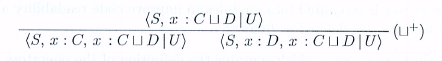
\includegraphics[scale=0.25]{img/union_rule.png}\end{center} %%FIXME: ripristinare l'albero!
%	\begin{prooftree}
%		\rootAtTop
%		\AxiomC{$\langle S,\, x : C,\,x\,: C \sqcup D\,|\,U \rangle$}
%		\AxiomC{$\langle S,\, x : D,\,x\,: C \sqcup D\,|\,U \rangle$}
%		\RightLabel{$(\sqcup^+)$}
%		\BinaryInfC{$\langle S,\, x\,: C\sqcup D\,|\,U \rangle$}
%	\end{prooftree}
	\begin{flushright}if $x : C \notin S$ and $x : D \notin S$.\\\end{flushright}
	\caption{$\primo$ rule for $(\sqcup^+)$ and its precondition.}
	\label{fig_union_rule}
\end{figure}

This is how the theorem prover works on such a rule:

\begin{itemize}
\item First, it checks if the list $S$ contains a formula $x : C \sqcup D$;
\item If the answer is \emph{no}, it skips the rule and tries another one;
\item If the answer is \emph{yes}, it checks the precondition specified in figure \ref{fig_union_rule};
\item If the precondition is satisfied, it calls \texttt{prove/6} recursively two times, one for each conclusion.
\end{itemize}

\newpage


This is translated in the following Prolog code:

\begin{lstlisting}[caption={alct1.pl}, label={lst:zaino}, firstnumber=175]
/* or + */
prove(S,U,Lt,Labels,ABOX,Tree) :-
    member([X,C or D],S),
    \+(member([X,C],S)),
    \+(member([X,D],S)),!,
    /* build the lists for the left and right sub-trees */
    prove([[X,C]|S],U,Lt,Labels,ABOX,Tree1),!,
    prove([[X,D]|S],U,Lt,Labels,ABOX,Tree2),!,
    buildTree('ph1','or+',S,U,[Tree1,Tree2],Tree),!.
\end{lstlisting}\vspace{0.5cm}

There is a small difference between how static and dynamic rules are implemented.

Static rules always introduce at most two branches in the proof tree (like in the previous example).

This is not true for dynamic rules where the number of branches varies depending on the number of labels present in the tree.

Figure \ref{fig_box_rule} shows an example.


\begin{figure}[htp]
\begin{center}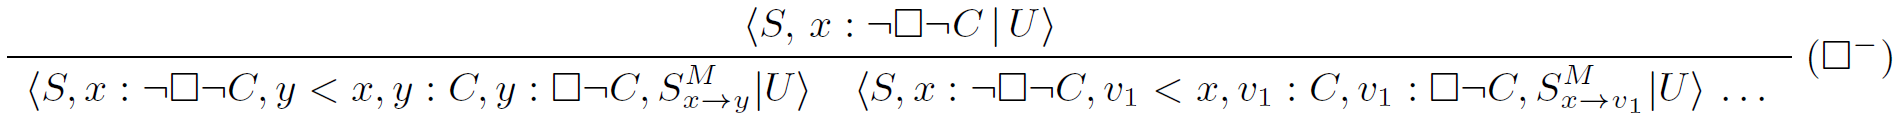
\includegraphics[scale=0.32]{img/box_rule.png}\end{center} %%FIXME: ripristinare l'albero!
%\footnotesize
%\begin{prooftree}
%	\rootAtTop
%	\def\defaultHypSeparation{\hskip .02in}
%	\AxiomC{$\langle S, x : \neg \Box \neg C, y < x, y : C, y : \Box \neg C, S^M_{x\rightarrow y}|U \rangle$}
%	\AxiomC{$\langle S, x : \neg \Box \neg C, v_1 < x, v_1 : C, v_1 : \Box \neg C, S^M_{x\rightarrow {v_1}}|U \rangle\,\dots$}
%	\RightLabel{$(\Box^-)$}
%	\BinaryInfC{$\langle S,\, x : \neg \Box \neg C\,|\,U \rangle$}
%\end{prooftree}
\begin{flushright} with $y$ fresh,\\
if $\not\exists z \prec x$ s.t. $z \equiv_{S,x:\neg \Box \neg C} x $ and $ \not\exists u$ t.c. $\{u < x, u : C, u : \neg \Box \neg C, S^M_{x\rightarrow u} \} \subseteq S$\\
$\forall v_i$ occurring in $S$.
\normalsize
\end{flushright}
	\caption{$\primo$ rule for $(\Box^-)$ and its precondition.}
	\label{fig_box_rule}
\end{figure}


An additional support predicate, called \texttt{proveRecB/10}, was introduced for each dynamic rule to manage the variable number of recursive calls.\\

As described in chapter \ref{tab}, the calculus is composed of two phases.

The first phase is implemented in the Prolog module \texttt{alct1} and can be started invoking the predicate \texttt{prove(S,U,F,Tree)}.

The Prolog interpreter then proceeds trying to apply rules of the first phase (corresponding to $\primo$), until the theorem is proved or a branch in the proof tree cannot be closed (i.e. no other rule in phase one can be applied). 
In this case, a verification by the second phase of the calculus ($\secondo$) must be undertaken by such open branch.

The implementation of $\secondo$ is coded in the module \texttt{alct2}, which exposes the predicate \texttt{prove\_phase2/6}.

\newpage


\chapter{The distributed theorem prover: DysToPic}\label{chap_dystopic}
\section{Background}\label{bg}
%%% distributed - parallel
%%%TODO: check!!!
With the increasing accessibility of multi--core processors and distributed computing networks, it has become imperative to investigate novel ways of using these concurrency and distribution technologies to tackle hard problems and to tap latent distribution and collaborative problem solving opportunities present in various tasks that computers are being used to solve.
Theorem proving, with its vast combinatorially explosive search spaces and increasingly complex and bigger problems, can benefit from these new ways of programming and new technologies \cite{conf/ieeehpcs/SripriyaBS09}.


This work investigates the application of a concurrent/collaborative approach to the pre--existing theorem prover called \emph{PreDeLo} (described in \ref{predelo}): the result is a new software solution, called \emph{DysToPic}, presented in the sequel.



%%\chapter{Architectural design}\label{arch}

\section{Our solution: the DysToPic system}

%%%TODO: Mettere in evidenza che si tratta del contributo originale

The main goal of our work is to improve the performances of the previously implemented theorem prover.
In the previous software \emph{PreDeLo}, especially when using $\alctmin$, the combination of an extremely high complexity of the calculus \footnote{In Theorem \ref{overall_complexity} we showed that the problem of deciding whether \emph{KB} $\models_{min}^{\ellet} F$ is in $\textsc{co-NExp}^\textsc{NP}$.} and the sequential implementation used to tackle it, can cause delays of several minutes before receiving a result even for small sized query formulas.
As we described previously, the calculus $\alctmin$ is not inherently sequential and can be effectively parallelised.

We therefore aim to build a distributed application for theorem proving in $\alctmin$, so that the computational burden can be spread amongst different machines, which can work in parallel.

\newpage

\section{A two--phase calculus}\label{calc_2ph}
For the sake of clarity we recall here that, as we described in detail in chapter \ref{tab}, $\nuovoc$ uses a tableaux calculus to verify whether a query entails from a knowledge base, i.e. $KB \models_{min} F$, which is equivalent to state that $F$ is verified in all the minimal models of the $KB$.\\
To do so, the calculus tries to build a model of $KB \unione \neg F$ (a counterexample). If it fails, then the query entails from the $KB$, otherwise it does not.\\

The process is designed as a two--phase calculus.

The first phase generates models of $KB \unione \{\nott F\}$. The ones in which $F$ holds cannot be counterexamples, thus they are discarded. A model $\emme_i$ of $KB \unione \{\nott F\}$ in which $F$ does not hold, instead, could be a counterexample: it is considered promising and will be further verified by the second phase of the calculus.\\
The second phase, indeed, uses $\secondo$: in order for a model $\emme_i$ of $KB \unione \{\nott F\}$ to be a counterexample of the entailment, it has to be a $minimal$ model of the $KB$. As stated in section \ref{tableau_ph2}, this means that, for each candidate model $\emme_i$, the second phase tries to build a model of the $KB$, $\emme_j^{KB}$, which is preferred to $\emme_i$. If every attempt of the second phase fails (i.e. no $\emme_j^{KB} \prec \emme_i$), then that candidate $\emme_i$ is the minimal model (i.e. the counterexample): this means that $KB \models_{min} F$.
Conversely, in case even a single $\emme_j^{KB}$ is found to be preferred to an $\emme_i$, that $\emme_i$ cannot be the counterexample.
If every $\emme_i$ has at least one corresponding $\emme_j^{KB}$ so that $\emme_j^{KB} \prec \emme_i$, then the whole research for a counterexample has failed, which means that $KB \unione \neg F$ has no models, and $KB \models_{min} F$.\\

%%%TODO: fare un disegno (eventualmente riciclare lo schema dell'esempio)
%% qui quello che raccontiamo è il funzionamento: mostrare lo schema di una situazione in cui è stato generato un alberello
%% > questo ramo resta aperto e non trova la contraddizione e parte fase2 e ciascuno genera un alberello
%%   A QUESTO PUNTO: cosa fa predelo vs. cosa fa il mio <- dev'essere evidente il passo avanti che ho fatto con la mia soluzione
%%
%% 

This procedure can be seen as the generation and traversal of a tree.

The first phase generates branches \textbf{B}$_i$, corresponding to models $\emme($\textbf{B}$_i)$, and uses $\primo$ to accept or refuse them.
A branch is considered $open$ until it is verified and, if it does not represent a counterexample, it is $closed$. The branches which are still \emph{open} after the first phase require further verification by $\secondo$, therefore they will be processed by the second phase.

As we showed in \ref{predelo_execution}, \emph{PreDeLo} was forced to immediately verify with $\secondo$ each branch generated by $\primo$, sequentially, interrupting de facto $\primo$.

In this section, instead, we explain that there is no need for the first phase of the calculus to wait for the result of one elaboration of the second phase on an open branch, before generating another candidate branch.

Indeed, in order to prove whether a query entails from a $KB$, the first phase can be executed on a machine; every time that a branch remains open after the first phase, the execution of the second phase for this branch can be performed in parallel, on a different machine.
Meanwhile, the main machine, instead of waiting for the termination of the second phase on that branch (as it happened in the sequential implementation of \emph{PreDeLo}), can carry on with the computation of the first phase (potentially generating other branches).

If, after the verification of the second phase, a branch remains open, then the whole entailment cannot be satisfied (we have therefore found a counterexample), so the computation process can be interrupted early.

This way, if the first phase reaches the end of its computation (meaning that it has generated every candidate model of the $KB$), it doesn't have to wait for the ``answers'' of each second phase in every case:
\begin{itemize}
\item if all the branches generated in the first phase remain open (i.e. all the branches generated in the second phase answer \emph{yes}), then the theorem prover answers \emph{yes} (which means the query entails from the $KB$);
\item if any of them is closed (i.e. any branch generated in the second phase answers \emph{no}), the global answer is \emph{no} (which means the query does not entail from the $KB$).
\end{itemize}

%%% worker - employer
%%%TODO: check!!!
\section{Worker-employer}\label{workemp}

In order to describe the software architecture that we have developed, we refer to the \emph{worker}-\emph{employer} metaphor.

The system is composed of:
\begin{itemize}
\item a single \emph{employer}, which is in charge of verifying the query and yielding the final result. It also implements the first phase of the calculus and uses $\primo$ to generate the various \emph{parallel branches}: the ones that it cannot close, it passes to a \emph{worker};
\item an unlimited number of \emph{workers}, which use $\secondo$ to evaluate the models generated by the \emph{employer};
\item a \emph{repository}, which stores all the answers coming from the \emph{workers}.
\end{itemize}

\newpage

Figure \ref{DIAG_1} shows us a high--level representation of the system.

\begin{figure}[H]
\centering
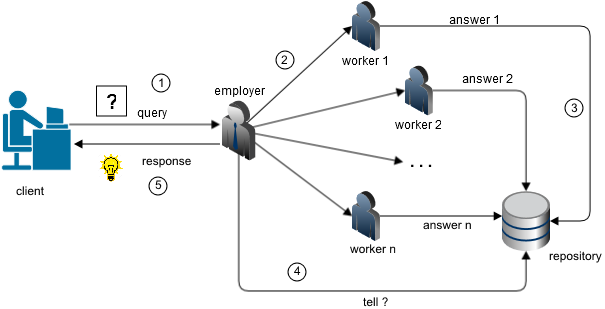
\includegraphics[scale=.9]{img/DIAG_1.png}
\caption{}
\label{DIAG_1}
\end{figure}

When presented with a query \circled{1}, the employer begins to analyse it through the first phase of the calculus.
If, during the computation of the first phase calculus, the \emph{employer} needs to verify a \emph{parallel branch} via the second phase calculus, it delegates it to one of the registered \emph{workers} \circled{2}, and consequently proceeds with its calculations on other branches.

When a \emph{worker} terminates its execution, it reports its result to the \emph{repository} \circled{3}.

The \emph{employer} has to keep a continuous dialogue with the \emph{repository} \circled{4}:
\begin{itemize}
\item if every branch has been processed and each worker has answered affirmatively, the employer can conclude that the query does entail from the \emph{KB};
\item otherwise, since a single negative answer from a \emph{worker} can invalidate the whole entailment, the \emph{employer} can conclude the proof as soon as the first negative answer comes into the \emph{repository}.
\end{itemize}
The execution ends when the response (``YES'' or ``NO'') is presented to the client \circled{5}.

\newpage

\section{Technologies used}\label{tech}

%%%%%%%%%%%% SICSTUS %%%%%%%%%%%%%%%%%%%%%

\subsection{Calculus implementation - SICStus Prolog}

Prolog is a declarative programming language developed at the University of Marseille, as a practical tool for programming in logic. The program logic is expressed in terms of relations, represented as facts and rules. A computation is initiated by running a query over these relations\cite{Lloyd:1984:FLP:2214}.

SICStus is a Prolog system developed at the Swedish Institute of Computer Science. Parts of the system were developed by the project “Industrialization of SICStus Prolog” in collaboration with Ericsson Telecom AB, NobelTech Systems AB, Infologics AB and Televerket\cite{sicstus_intro}.\\

Both the employer and the workers of our system rely on Prolog for their computing cores: respectively \verb$alct1.pl$ and \verb$alct2.pl$. The former implements the first phase ($\primo$), while the latter implements the second phase of the calculus ($\secondo$).

%%%%%%%%%%%% JASPER %%%%%%%%%%%%%%%%%%%%%

\subsection{Interface between Prolog and Java - Jasper}\label{ssec_jasper}

Jasper is a bi-directional interface between Java and SICStus. The Java-side of the interface consists of a Java package (\verb$se.sics.jasper$) containing classes representing the SICStus runtime system (\verb$SICStus$, \verb$SPTerm$, etc). The Prolog part is designed as a library module (\verb$library(jasper)$).

The library module \verb$library(jasper)$  provides functionality for controlling the loading and unloading the JVM (Java Virtual Machine), method call functionality (\verb$jasper_call/4$), and predicates for managing object references.

Jasper can be used in two modes, depending on which system acts as \emph{parent application}.
\begin{enumerate}
\item[(case 1)] If Java is the parent application, the SICStus runtime kernel will be loaded into the JVM using the \verb$System.loadLibrary()$ method (this is done indirectly when instantiating a SICStus object). In this mode, SICStus is loaded as a runtime system.

\item[(case 2)] If SICStus is the parent application, Java will be loaded as a foreign resource using the query \verb$use_module(library(jasper))$. The Java engine is initialized using \verb$jasper_initialize/[1,2]$\cite{sicstus_jasper}.\\
\end{enumerate}

Our implementation uses both of these modes, with the purpose of decoupling the two phases of the calculus.

\newpage

The \emph{employer} handles the query in \verb$Phase1Thread.java$, a piece of Java code which presents it to \verb$alct1.pl$, the Prolog core implementing $\primo$ (case 1).

\begin{lstlisting}[caption={Phase1Thread.java}, label={lst:phase1t}, firstnumber=27]
// Creates a new SICStus object.
SICStus sp = new SICStus();
	
// Loads the prolog implementation of the tableau for
// the first phase of the calculus.
sp.load("alct1.pl");
	
Map<String, SPTerm> map = new HashMap<String, SPTerm>();
	
// Makes the SICStus object open the query.
Query query = sp.openPrologQuery(queryString, map);
\end{lstlisting}\vspace{0.5cm}

Every time that an open branch is generated, \verb$alct1.pl$ calls (case 2) \verb$Phase1RMIStub.java$, another piece of Java code which will send it to the correct \emph{worker}.

\begin{lstlisting}[caption={alct1.pl}, label={lst:alct1}, firstnumber=293]
jasper_call(JVM,
	method('employer/Phase1RMIStub', 'solveViaRMI', [static]),
	solve_via_rmi(+chars, +chars),                      
	solve_via_rmi(NextWorkerName, OpenBranch) ),!.
\end{lstlisting}\vspace{0.5cm}

The \emph{workers} will then have to process the open branches with $\secondo$, which is implemented in \verb$alct2.pl$. They will do so in \verb$SolverThread.java$ (case 1).

\begin{lstlisting}[caption={SolverThread.java}, label={lst:solvert}, firstnumber=22]
Query query = sp.openPrologQuery(remoteQuery, map);

// Verifies whether the query can be solved.
if (query.nextSolution()) {
	// If so, asks the repository to store a positive answer.
	repository.store(true);
} else {
	// Otherwise, asks the repository to store a negative answer.
	repository.store(false);
}
query.close();
\end{lstlisting}\vspace{0.5cm}

%%%%%%%%%%%% CONCURRENCY %%%%%%%%%%%%%%%%%%%%%

\subsection{Concurrency - Java threads}
Parallel computing is a form of computation in which many calculations are carried out simultaneously, operating on the principle that large problems can often be divided into smaller ones, which are then solved concurrently (``in parallel'')\cite{Almasi:1989:HPC:160438}.

The Java platform is designed from the ground up to support concurrent programming, with basic concurrency support in the Java programming language and the Java class libraries. Since version 5.0, the Java platform has also included high-level concurrency APIs\cite{oracle_thread}.

Concurrency is the main goal of our implementation, since we want the execution of the first phase of the calculus to be independent from the second. Java natively supports concurrency via multithreading.\\

The \emph{employer} uses a separate thread (implemented in \verb$Phase1Thread.java$) to perform the actual invocation of $\primo$ on the query, while its main thread polls the \emph{repository} waiting for termination\footnote{Let us recall the reader that a global termination can be reached when the first counterexample is found, even if not all of the branches have been explored.}.

\begin{lstlisting}[caption={Employer.java}, label={lst:employer}, firstnumber=116]
// Spawns a new thread which launches the first phase of the calculus
Thread phase1Thread = new Thread(new Phase1Thread(queryString));
phase1Thread.start();

Repository repository = (Repository) registry.lookup("Repository");
		
// The employer now polls the repository until it has at least one answer.
while (true) {
	...
	if (repository.tell())
		System.out.println("YES, inference done.");
	else
		System.out.println("NO, inference failed.");
}
\end{lstlisting}\vspace{0.5cm}

\newpage

During $\primo$, every time that the \emph{employer} wants to ask a \emph{worker} to verify a branch (this happens in \verb$Phase1RMIStub.java$), a new thread is spawned (\verb$PrologWorker.java$).

\begin{lstlisting}[caption={Phase1RMIStub.java}, label={lst:phase1rmi}, firstnumber=68]
// Spawns a new thread, asking it to solve the query.
Thread t = new Thread(new PrologWorker(worker, query));
t.start();

// Increments the counter of the queries which have been asked.
c.increment();
\end{lstlisting}\vspace{0.5cm}

The \emph{worker} itself uses threads: its main thread (\verb$Phase2Worker.java$) simply enqueues each request coming from the \emph{employer} (in \verb$Solver.java$) and spawns a new thread, \verb$SolverThread.java$, which performs $\secondo$.

\begin{lstlisting}[caption={Solver.java}, label={lst:solver}, firstnumber=38]
solverThread = new Thread(new SolverThread(this.name, pendingRequests));
solverThread.start();
\end{lstlisting}\vspace{0.5cm}

%%%%%%%%%%%% RMI %%%%%%%%%%%%%%%%%%%%%

\subsection{System distribution - Java RMI}

%%TODO: mettere il codice significativo! === mostrare soprattutto i punti di distacco da quello di adam

The Java Remote Method Invocation (Java RMI) is a Java API that performs the object-oriented equivalent of remote procedure calls (RPC), with support for direct transfer of serialized Java classes and distributed garbage collection \cite{rmi}.
It enables to create distributed Java applications, in which the methods of remote objects can be invoked from other Java virtual machines, possibly on different hosts\cite{oracle_rmi}.

As stated in \ref{ssec_jasper}, since \emph{DysToPic} relies on a Java interface to Prolog, it was natural to design the distribution feature around Java APIs, too\footnote{With Java versions before Java 5.0 developers had to compile RMI stubs in a separate compilation step using \texttt{rmic}. Version 5.0 of Java and beyond no longer require this step.}.

The RMI architecture makes use of a \emph{Registry} (\verb$java.rmi.registry.Registry$) that provides methods for storing (methods \texttt{bind}, \texttt{unbind}, \texttt{rebind}) and retrieving (methods \texttt{list} and \texttt{lookup}) remote object references bound with arbitrary string names.\\

\newpage

The \emph{repository} (which runs on the same machine as the \emph{employer}) will begin its execution by asking the RMI registry to bind itself (\verb$AnswersRepository.java$) as ``Repository''.

\begin{figure}[H]
\centering
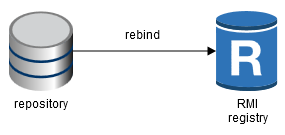
\includegraphics[scale=.7]{img/DIAG_11.png}
\caption{}
\label{}
\end{figure}

Due to a limitation in the RMI protocol, we had to make the repository expose a method called \texttt{proxyRebind(String name, Remote stub)}, which binds the Remote object that is supplied to it to the local RMI registry, with the selected \texttt{name}
\footnote{This is required since by default one cannot bind a service on a RMI registry which is on a remote machine.}.

Each \emph{worker} then asks the RMI registry to lookup for the \emph{repository} (steps \circled{1} and \circled{2}) and uses \texttt{proxyRebind} to bind itself (steps \circled{3} and \circled{4}) to the RMI registry as \texttt{"Worker*"}, where \texttt{*} is any string, e.g. both \texttt{"Worker1"} and \texttt{"WorkerFoo"} are valid names.

\begin{figure}[H]
\centering
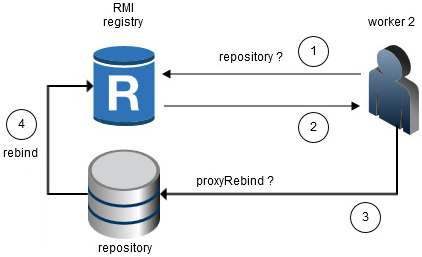
\includegraphics[scale=.8]{img/DIAG_13.png}
\caption{}
\label{}
\end{figure}

When the \emph{employer} starts, it retrieves the list of all the \emph{workers} which are currently bound to the RMI registry and consults it every time it needs a \emph{worker}.

\begin{figure}[H]
\centering
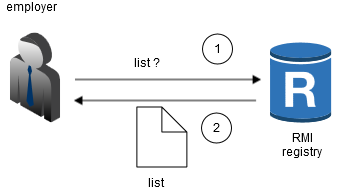
\includegraphics[scale=.8]{img/DIAG_12.png}
\caption{}
\label{}
\end{figure}

\section{An example of execution}\label{example}
\begin{enumerate}

\item The RMI registry is launched on the machine `A' on port `x': every other machine will have to perform their requests to it.

\begin{figure}[htp]
\centering
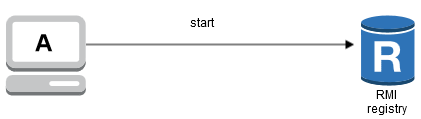
\includegraphics[scale=.9]{img/DIAG_2.png}
\caption{}
\label{}
\end{figure}

\item The repository (\texttt{AnswersRepository.java}) is then executed on the same machine. It binds itself on the RMI registry as ``Repository''.

\begin{figure}[htp]
\centering
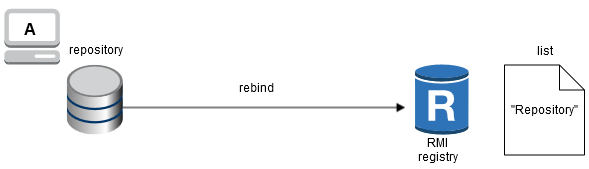
\includegraphics[scale=.9]{img/DIAG_3.png}
\caption{}
\label{}
\end{figure}

\newpage

\item Then an arbitrary number of workers (\texttt{Phase2Worker.java}) is launched on an arbitrary number of machines (let's say machines `B' to `N') - for instance, one worker per CPU\footnote{We chose to use the convention that each worker has a different name, which has to be a string starting with ``Worker'' (i.e. ``Worker1'' ``Worker2'', and so on).}.

\begin{figure}[H]
\centering
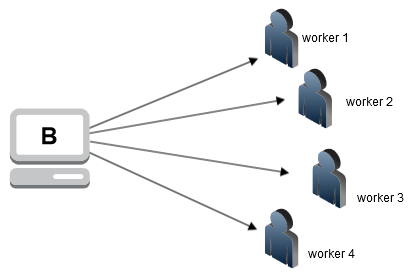
\includegraphics[scale=.6]{img/DIAG_4.png}
\caption{}
\label{}
\end{figure}

Each worker binds itself to the RMI registry (through the \texttt{proxyRebind} method of \texttt{AnswersRepository.java} - steps \circled{1} to \circled{4} in figure \ref{DIAG_5}) and then starts its single instance of \texttt{SolverThread} (step \circled{5}).

\texttt{SolverThread.java} creates a SICStus object with the code of \texttt{alct2.pl} (which corresponds to $\secondo$) and then waits until a request (an object of class \texttt{Request.java}) comes from the employer.

\begin{figure}[H]
\centering
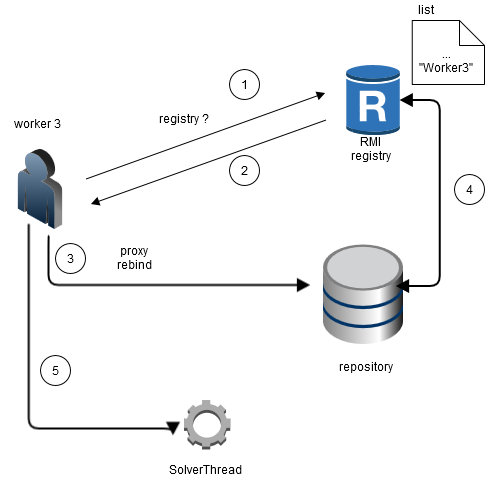
\includegraphics[scale=0.75]{img/DIAG_5.png}
\caption{}
\label{DIAG_5}
\end{figure}

\item Afterwards, the \emph{employer} (\texttt{Emloyer.java}) is started on the machine `A', and \circled{1} receives from the user a \texttt{queryString} (which contains both the $KB$ and the actual query to be verified). It retrieves a list of each worker bound to the RMI registry (steps \circled{2} and \circled{3}) and (step \circled{4}) writes it onto a file (\texttt{workersList.txt} - this file is the means for communicating the names to \texttt{alct1.pl}).

\begin{figure}[H]
\centering
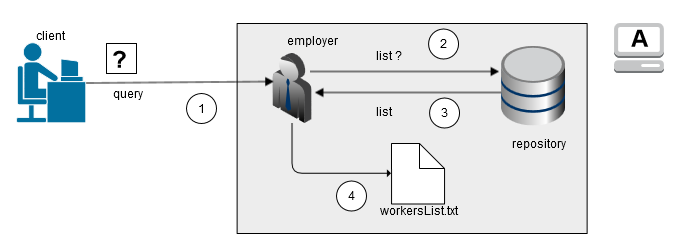
\includegraphics[scale=.7]{img/DIAG_6.png}
\caption{}
\label{}
\end{figure}

[The following description refers to figure \ref{DIAG_7} on page \pageref{DIAG_7}.]

\item[5a.] Then the \emph{employer} spawns a new thread, \texttt{Phase1Thread.java} \circled{1}.

This creates a SICStus object and loads it with the code of \texttt{alct1.pl}, which contains the rules of $\primo$. Then the \texttt{queryString} is passed \circled{2} to this SICStus object as a parameter (via Jasper). The query is executed and the control passes to the Prolog code (\texttt{alct1.pl}), which starts manipulating the \texttt{queryString} and generating various branches \circled{3}. Some may be closed (a), others may be open (b):
	\begin{itemize}
	\item If every generated branch is found to be closed, the computation can end with an affirmative answer: the query does entail from the $KB$.
	\item Otherwise, for each \emph{open} branch found, \texttt{alct1.pl} invokes (via Jasper) the method \texttt{solveViaRMI(String workerName, String query)} - this happens in  \texttt{Phase1RMIStub.java} \circled{4}. The \texttt{query} corresponds to the branch to be verified, while the \texttt{workerName} is extracted from the file \texttt{workersList.txt}\footnote{This is done FIFO, reading a name from the top of the file, and writing it on the bottom, and allows a simple form of load balancing.}.
	\end{itemize}
	
\texttt{Phase1RMIStub.java}'s main thread, then \circled{5} spawns a new thread (\texttt{PrologWorker.java}) and \circled{6} increases the counter of the open branches (an object of class \texttt{Counter.java}).

An object of class \texttt{PrologWorker.java} allows the \emph{employer} to use a \emph{worker}'s method, \texttt{solve}\footnote{In the distributed computing environment, the server-side object participating in the distributed object communication is called a \emph{skeleton}, while the client-side object is called a \emph{stub}. In this particular case, the \emph{worker} is the server, so the method is specified in the \emph{skeleton} and the employer calls it on its \emph{stub}.}, which the \emph{employer} can use to solve the query, i.e. to ask the \emph{worker} to use $\secondo$ to verify whether the branch is \emph{open} or \emph{closed}.

\begin{figure}[H]
\centering
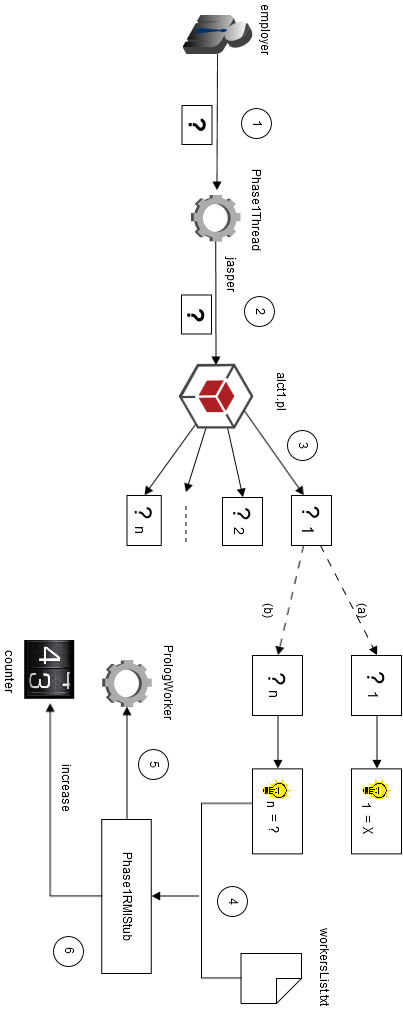
\includegraphics[scale=.7]{img/DIAG_7.png}
\caption{}
\label{DIAG_7}
\end{figure}

\newpage

\item[5b.] Meanwhile, as we can see in figure \ref{DIAG_8}, the \emph{employer}'s main thread (just after spawning \texttt{Phase1Thread.java}) enters a loop in which it polls the \emph{repository} until a global answer can be found. This happens when:
\begin{itemize}
\item one \emph{worker} has answered \texttt{false}, invalidating the whole entailment (i.e. the method \texttt{tell} returns \texttt{false}) - here the \emph{employer} answers 'NO';
\item all the open branches (counted by \texttt{Counter.java}) have been tested and every \emph{worker} has answered \texttt{true} (the method \texttt{tell} still returns \texttt{false}) - here the \emph{employer} answers 'YES'.
\end{itemize}
Until then, the \emph{employer} just remains in a busy wait condition.

\begin{figure}[H]
\centering
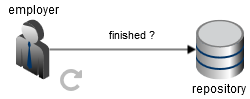
\includegraphics[scale=1.00]{img/DIAG_8.png}
\caption{}
\label{DIAG_8}
\end{figure}

\newpage

\item[6a.]When the \texttt{PrologWorker} thread of the \emph{employer} calls \texttt{solve(String remoteQuery)} on a \emph{worker}, for instance ``Worker2'' on machine `B' (steps \circled{1} to \circled{3}), the \emph{worker} simply asks its solver object (class \texttt{Solver.java}) to enqueue the request \circled{4}.

\begin{figure}[H]
\centering
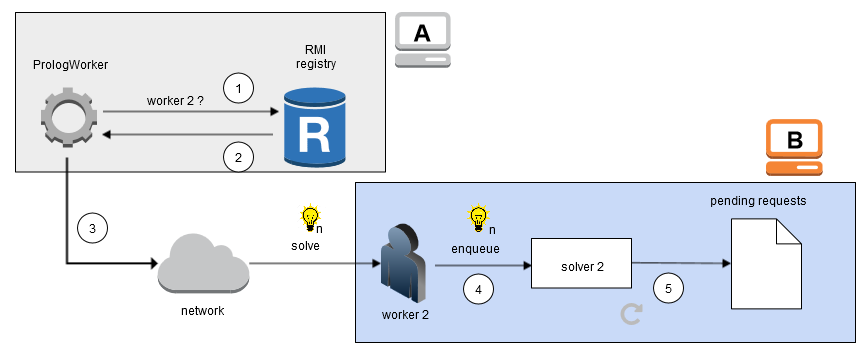
\includegraphics[scale=.70]{img/DIAG_9.png}
\caption{}
\label{DIAG_9}
\end{figure}

The \texttt{SolverThread} will then take the request from the queue and elaborate it through \texttt{alct2.pl} (steps \circled{5} to \circled{8}).
This elaboration yields an answer of the form \texttt{true} or \texttt{false} \circled{9}, which is then sent (through the method \texttt{store(Boolean answer)}) to the repository (steps \circled{10} to \circled{12}). The \texttt{SolverThread} then restarts its infinite loop and looks for another request that may or may not have come from the \emph{employer} in the meantime.

\begin{figure}[H]
\centering
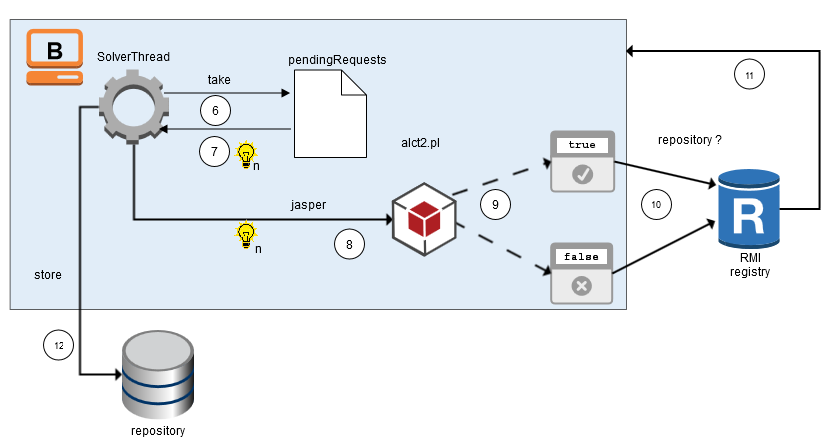
\includegraphics[scale=.70]{img/DIAG_10.png}
\caption{}
\label{DIAG_10}
\end{figure}

\end{enumerate}

%%%TODO: Sezione test
%indicare che sono risultati ampiamente preliminari
% dire che in ogni caso non differisce dalle prestazioni della versione di adam (a meno di overhead)
% dire che anche il generatore casuale è poco raffinato

\newpage

\chapter{Preliminary performance testing}\label{testing}

We have made a preliminary attempt to show how \emph{DysToPic} performs, especially in comparison with \emph{PreDeLo}.\\

Due to the novelty of the $\alctmin$ language, there are no public KBs available for testing purposes.

A draft of an automated random generator of KBs (and queries) was developed for \emph{PreDeLo}.
We can confirm that the data that it produces are still compatible with \emph{DysToPic}, although the generator itself calls for further analysis. This is outside the scope of this thesis.

This chapter is far from being an exhaustive verification; however we can already say that the results for our prover are at the very least comparable with those obtainable by \emph{PreDeLo}.
In the sequel we will illustrate both some interesting test cases and the environment in which the tests were performed.

\section{Hardware and software platforms}

\subsection{Software}

Both \emph{PreDeLo}'s and \emph{DysToPic}'s Prolog cores have been compiled with SICStus 4.1.1 (version x86\_64-linux-glibc2.7).

Due to compatibility reasons between Java and SICStus (via the Jasper library), the Java applications had to be developed using the Java 6 platform (we used the javac compiler at version 1.6.0\_32)\footnote{Newer versions of SICStus have been released which are compatible with Java 7, although they require a new license.}.



\newpage

\subsection{Hardware}\label{hardware}
The machines used for our tests are:

\begin{itemize}

\item \textbf{ninjavm}: a desktop PC with 

CPU: Intel Core i5-3570K (3.4-3.8GHz, 6MB L3 cache) - 4 cores, 4 threads;\\
RAM: 8GB\\
running Ubuntu 14.04.1 64 bit OS (kernel 3.13.0-35) in a virtual machine, with 2 available virtual cores and 4GB of available RAM; the host OS is Windows 7.

\item \textbf{evo}: another desktop PC with

CPU: Intel Pentium G2030 (3.0GHz, 3MB L3 cache) - 2 cores, 2 threads;\\
RAM: 4GB\\
running natively Ubuntu 14.04.1 64 bit OS (kernel 3.13.0-29)

\item \textbf{x220}: a Lenovo X220 laptop with

CPU: Intel Core i7-2640M (2.8-3.5GHz, 4MB L3 cache) - 2 cores, 4 threads;\\
RAM: 8GB\\
running natively Ubuntu 14.04.1 64 bit OS (kernel 3.13.0-35)


\item \textbf{x230vm}: a Lenovo X230 laptop with

CPU: Intel Core i7-3520M (2.9-3.6GHz, 4MB L3 cache) - 2 cores, 4 threads;\\
RAM: 8GB\\
running Ubuntu 14.04.1 64 bit OS (kernel 3.13.0-35) in a virtual machine, with 2 available virtual cores and 4GB of available RAM; the host OS is Windows 7.

\end{itemize}

All are fairly recent machines and can be considered almost equal in terms of calculating capacity.
The following results have been obtained with each machine connected to a LAN over a domestic router, via Ethernet links at 100 Mbit/s.

\newpage

\section{Expectations}\label{expectations}
Following what we stated in \ref{calc_2ph}, we recall that the possible outcomes of an execution of $\nuovoc$ on a query are:
\begin{enumerate}
\item an immediate \emph{YES} at the end of the first phase ($\primo$), without need of any verification with the second phase ($\secondo$).

This can happen in case the query is trivially true or the KB is inconsistent;

\item a global \emph{NO}, which requires that at least one \emph{worker} had answered \texttt{"false"} to an open branch;

\item a global \emph{YES}, which requires that every \emph{worker} had answered \texttt{"true"} to every open branch
\footnote{Our tests seem to suggest that the random generator described at the beginning of chapter \ref{testing} cannot generate examples of case 3. Further investigation of this issue is required before drawing definitive conclusions. We reaffirm that this is outside the scope of this work.}
.
\end{enumerate}

Clearly we know that the increased parallelism achieved by \emph{DysToPic} comes at the price of an initial overhead required for the set--up of the various distributed components of its architecture.
\emph{DysToPic} uses the \emph{repository} as a form of shared memory for the partial results, which can also be a source of slowdowns.
Moreover, it is clear that the responses will take some time to come from the remote \emph{workers} to the local \emph{repository}.

For these reasons, we obviously expect the queries of case 1. (immediate \emph{YES}) to be resolved faster by \emph{PreDeLo}.

In general, we also expect that this overhead can cause \emph{PreDeLo} to have a bit of advantage in case the  query requires only a small amount of running time.

The cases 2. and 3. are instead more promising for \emph{DysToPic}: its parallelism can be fully exploited when case various branches require the verification of the second phase.

\newpage

\section{Experimental results}

\subsection{Naming convention}

Obviously, since \emph{PreDeLo} is a sequential program, it can be only executed on a single machine; we tested it only on \textbf{ninjavm}.\\

On the other hand, \emph{Dystopic} was tested in various configurations.
While both the \emph{employer} and the \emph{repository} were always executed on \textbf{ninjavm}, in the sequel we call:

\begin{itemize}

\item \textbf{2W} a configuration in which 2 \emph{workers} were executed on \textbf{ninjavm};
\item \textbf{4W} a configuration in which 2 \emph{workers} were executed on \textbf{ninjavm} and 2 on \textbf{evo};
\item \textbf{8W} a configuration in which 2 \emph{workers} were executed on \textbf{ninjavm}, 2 on \textbf{evo} and 4 on \textbf{x220};
\item \textbf{10W} a configuration in which 2 \emph{workers} were executed on \textbf{ninjavm}, 2 on \textbf{evo}, 4 on \textbf{x220} and 2 on \textbf{x230vm}.

\end{itemize}

As we showed in section \ref{hardware}, some of the machines are actually virtualised, although we limited the amount of \emph{workers} per machine, so that each machine has exactly one \emph{worker} per logical thread.

\newpage


\subsection{Comparison of running times}

\subsubsection{Query 1: answer YES (case 1)}
%BIRDS4#prove([ [[tweety,1],bird], [[tweety,1],penguin] ], [ [[ti bird inc flying],[]], [[penguin inc bird],[]], [[penguin inc neg flying],[]] ], [[tweety,1],neg flying], Tree).

This query does not produce any open branch in $\primo$.\\

\begin{tabular}{ll}
	\textbf{ABox} & \textbf{TBox}\\
	$Bird(tweety)$ & $\tip(Bird) \sqsubseteq FlyingAnimal$\\
	$Penguin(tweety)$ & $Penguin \sqsubseteq Bird$\\
	& $Penguin \sqsubseteq \neg FlyingAnimal$\\[0.5cm]
\end{tabular}

\begin{tabular}{ll}
\textbf{Query} & \textbf{Result}\\
$\neg FlyingAnimal(tweety)?$ & YES\\
\end{tabular}

\begin{figure}[ht]
\begin{bchart}[step=200,max=200,unit=ms,scale=1.4]
	\bcbar[label=PreDeLo, value=2]{2}
    \medskip
    \bcbar[label=2W, value=124]{124}
    \medskip
    \bcbar[label=4W, value=124]{124}
    \medskip
    \bcbar[label=8W, value=126]{126}
    \medskip
    \bcbar[label=10W, value=127]{127}
\end{bchart}
\caption{}
\end{figure}

This chart shows us that, in this first case, the set--up overhead dominates the running time of \emph{DysToPic}: the query can be easily solved by $\primo$ and \emph{PreDeLo} does it more efficiently.

On the other hand, from a practical point of view, there is no noticeable difference between the running times of both theorem provers.

We can also notice how a small amount of time is required to start the various \emph{workers}.

\newpage

\subsubsection{Query 2: answer NO (case 2)}
%prove([[[mario,1], student],[[mario,1],workingStudent],[[mario,1],father], [[mario,1],tall] ],
%     [  [[ti student inc neg taxPayer],[]],[[workingStudent inc student],[]], [[ti workingStudent inc taxPayer],[]]   ],       [[mario,1], neg taxPayer],Tree).

This query generates 1 open branch in $\primo$, which has to be tested by a single \emph{worker} in $\secondo$.\\

\begin{tabular}{ll}
	\textbf{ABox} & \textbf{TBox}\\
	$Student(mario)$ & $\tip(Student) \sqsubseteq \neg IncomeTaxPayer$\\
	$WorkingStudent(mario)$ & $WorkingStudent \sqsubseteq Student$\\
	$Tall(mario)$ & $\tip(WorkingStudent) \sqsubseteq IncomeTaxPayer$\\[0.5cm]
\end{tabular}

\begin{tabular}{ll}
\textbf{Query} & \textbf{Result}\\
$\neg IncomeTaxPayer(mario)?$ & NO\\
\end{tabular}


\begin{figure}[ht]
\begin{bchart}[step=200,max=200,unit=ms,scale=1.4]
	\bcbar[label=PreDeLo, value=2]{2}
    \medskip
    \bcbar[label=2W, value=164]{164}
    \medskip
    \bcbar[label=4W, value=173]{173}
    \medskip
    \bcbar[label=8W, value=180]{180}
    \medskip
    \bcbar[label=10W, value=179]{179}
\end{bchart}
\caption{}
\end{figure}

The same considerations done for the previous chart still hold in this case.

Even if a branch requires further verification by $\secondo$, this requires very little effort (it takes less than 2 ms if done sequentially) and the running time is still widely dominated by the overhead.

However, \emph{DysToPic} is not noticeably slower than \emph{PreDeLo}.

\newpage

\subsubsection{Query 3: answer YES (case 3)}

This query generates 2 open branches in $\primo$, which have to be tested by the \emph{workers} in $\secondo$.\\

\begin{tabular}{ll}
	\textbf{ABox} & \textbf{TBox}\\
	$Student(mario)$ & $\tip(Student) \sqsubseteq \neg IncomeTaxPayer$\\
	$WorkingStudent(mario)$ & $WorkingStudent \sqsubseteq Student$\\
	$Tall(mario)$ & $\tip(WorkingStudent) \sqsubseteq IncomeTaxPayer$\\[0.5cm]
\end{tabular}

\begin{tabular}{ll}
\textbf{Query} & \textbf{Result}\\
$IncomeTaxPayer(mario)?$ & YES\\
\end{tabular}

\begin{figure}[ht]
\begin{bchart}[step=300,max=300,unit=ms,scale=1.4]
	\bcbar[label=PreDeLo, value=66]{66}
    \medskip
    \bcbar[label=2W, value=215]{215}
    \medskip
    \bcbar[label=4W, value=225]{225}
    \medskip
    \bcbar[label=8W, value=238]{238}
    \medskip
    \bcbar[label=10W, value=243]{243}
\end{bchart}
\caption{}
\end{figure}

This chart confirms that two, ``easy'', open branches are still not enough for \emph{DysToPic} to take advantage of its parallelism; the running times are a bit longer for \emph{PreDeLo}, but still nothing noticeable happens.\\

In general, we can make a query more complicate in various ways, for instance by adding elements to both the ABox or the TBox, or increasing the degree of nesting in the inclusions in the TBox.

We decided to test how each theorem prover reacted to a query which is substantially identical to the previous one, but with a larger KB.

In section \ref{alctmin} (Definition \ref{LogicalConsequenceALCTMIN}), we showed how adding \emph{irrelevant} assertions does not modify the result of the entailment.
Though, as we can see from the results, this comes at the cost of a larger number of open branches generated by $\primo$.

\subsubsection{Query 4: answer YES (case 3)}



This query generates 37 open branches in $\primo$, which have to be tested by the \emph{workers} in $\secondo$.\\

\begin{tabular}{ll}
	\textbf{ABox} & \textbf{TBox}\\
	$Student(mario)$ & $\tip(Student) \sqsubseteq \neg IncomeTaxPayer$\\
	$WorkingStudent(mario)$ & $WorkingStudent \sqsubseteq Student$\\
	$Tall(mario)$ & $\tip(WorkingStudent) \sqsubseteq IncomeTaxPayer$\\
	$Student(carlo)$ &\\
	$WorkingStudent(carlo)$ &\\
	$Tall(carlo)$ &\\[0.5cm]
\end{tabular}

\begin{tabular}{ll}
\textbf{Query} & \textbf{Result}\\
$IncomeTaxPayer(mario)?$ & YES\\
\end{tabular}

\begin{figure}[ht]
\begin{bchart}[step=5000,max=5000,unit=ms,scale=1.4]
	\bcbar[label=PreDeLo, value=4504]{4504}
    \medskip
    \bcbar[label=2W, value=3138]{3138}
    \medskip
    \bcbar[label=4W, value=2118]{2118}
    \medskip
    \bcbar[label=8W, value=2069]{2069}
    \medskip
    \bcbar[label=10W, value=1942]{1942}
\end{bchart}
\caption{}
\end{figure}

This is the first case in which \emph{DysToPic} can prevail; notice that the improvement is also visibly noticeable (in terms of seconds!).

The 37 open branches have to be verified sequentially by \emph{PreDeLo} and this clearly slows it down.
The fact that the performances of \emph{DysToPic} do not directly scale at the increase of the number of \emph{workers} may mean that one of these branches is more complex than the others, and its running time dominates the global result.

\newpage

\subsubsection{Query 5: answer YES (case 3)}

This query generates 1090 open branches in $\primo$, which have to be tested by the \emph{workers} in $\secondo$.\\

\begin{tabular}{ll}
	\textbf{ABox} & \textbf{TBox}\\
	$Student(mario)$ & $\tip(Student) \sqsubseteq \neg IncomeTaxPayer$\\
	$WorkingStudent(mario)$ & $WorkingStudent \sqsubseteq Student$\\
	$Tall(mario)$ & $\tip(WorkingStudent) \sqsubseteq IncomeTaxPayer$\\
	$Student(carlo)$ &\\
	$WorkingStudent(carlo)$ &\\
	$Tall(carlo)$ &\\
	$Student(giuseppe)$ &\\
	$WorkingStudent(giuseppe)$ &\\
	$Tall(giuseppe)$ &\\[0.5cm]
\end{tabular}

\begin{tabular}{ll}
\textbf{Query} & \textbf{Result}\\
$IncomeTaxPayer(mario)?$ & YES\\
\end{tabular}

\begin{figure}[ht]
\begin{bchart}[step=400,max=400,unit=s,scale=1.4]
	\bcbar[label=PreDeLo, value=370]{370}
    \medskip
    \bcbar[label=2W, value=210]{210}
    \medskip
    \bcbar[label=4W, value=112]{112}
    \medskip
    \bcbar[label=8W, value=95]{95}
    \medskip
    \bcbar[label=10W, value=82]{82}
\end{bchart}
\caption{Please note that this chart shows data measured in seconds,\\while the previous charts were measured in milliseconds.}
\end{figure}

Here, the improvement of \emph{DysToPic} is even more evident. We can see how the performance increase scales well up to 4 \emph{workers}. The improvement with more \emph{workers} is marginal, meaning that probably there are some branches that require prolonged running times.

%%%%%%%%%%%%%%%%%%%%%%%%%%%%%%%%%%%%%%%%%%%%%%%%%%%%%%%%%%%%%%
%%%%%%%%%%%%%%%%%%%%%%%  CONCLUSIONS  %%%%%%%%%%%%%%%%%%%%%%%%
%%%%%%%%%%%%%%%%%%%%%%%%%%%%%%%%%%%%%%%%%%%%%%%%%%%%%%%%%%%%%%
\chapter{Conclusions and future issues}

%%TODO: riassumere il mio contributo
% possiamo fare riferimento a cose già descritte all'interno
% 

%%TODO: mettere possibili sviluppi futuri

% si può estendere in particolare alle logiche a bassa complessità (citare articoli ?!?)

% aggiungere una section in cui si dice che il marchingegno è generalizzabile ai casi di DL-Lite, ad EL, ad altre DL con poco sforzo


% la mia architettura è applicabile ad un qualunque sistema di ragionamento (es a modelli minimali per logiche condizionali), ci saranno altri casi in cui una "fase1" genera varie "fasi2" che possono girare in parallelo, ad esempio tutti i meccanismi di ragionamento che implementano una semantica a modelli preferiti (esistono per circumscription, ecc IN LETTERATURA)


In this thesis we presented \emph{DysToPic}, a distributed theorem prover implementation for $\nuovoc$.\\


After describing the Description Logic $\mathcal{ALC}$, we showed how it was non--monotonically extended to obtain an expressive language for knowledge representation, $\alctmin$, for reasoning about prototypical properties and inheritance with exceptions.

Then we introduced the tableau calculus $\nuovoc$, presented in \cite{Giordano:2013:NDL:2435476.2435957}, which has been developed for deciding the satisfiability of $\alctmin$, and we discussed how the degree of expressiveness affects the decision complexity: the problem of deciding if a formula is minimally entailed respect to a $KB$ is in $\textsc{co-NExp}^\textsc{NP}$.
Such a high complexity classifies the problem itself as untreatable, nonetheless logics such as this are adopted in many real-life environments, thanks to various adaptations to the specific application environments, which provide approachable complexities. This shows us how even extremely complex problems can be treated, under specific conditions.\\

Since the previously developed theorem prover, \emph{PreDeLo}, showed the possibility of a mechanism of automated demonstration of complex formulas for this calculus, we decided to improve such approach.

\emph{DysToPic} is a Java software, built around two separate Prolog cores which implement the two phases of $\nuovoc$ ($\primo$ and $\secondo$). It relies on the RMI technology for the distribution of the calculus and it is multi--threaded for its parallelisation. This allows us to run the verifications (of the second phase) of multiple branches in parallel, on an unlimited number of machines at the same time, possibly finding a counterexample (in case of answer ``NO'') more rapidly.\\
Even if \emph{DysToPic}'s performances are promising, we intend to study further improvements through the application of refinements. We think that the first step in this direction should be the implementation of a query generator, to obtain a set of significant examples in order to perform further automatised performance tests.\\

\emph{DysToPic}'s system architecture has been designed to be as general as possible, in order to be open to further applications and improvements.\\
For instance, the adaptation of this software to the low complexity tableaux calculus $\calclite$ (the calculus corresponding to $DL-Lite_c\tip_{min}$), would be almost effortless; doing so we would sacrifice some language expressiveness as a tradeoff for the decreased complexity of the decision.

$DL-Lite$ and its related logic $\mathcal{EL}$ are specifically tailored for effective query answering over DL knowledge bases containing large amounts of data (e.g the GALEN medical knowledge base), and are applied in a wide range of fields.\\

Moreover, our distributed approach is conceptually general, and it could be adapted to various reasoning mechanisms: for instance, those which make use of a semantics with preferred models (e.g. for conditional logics \cite{jelia2012nmr}, or for circumscription \cite{hitzlertableau}, \cite{Voorbraak:1991:PMS:646559.695082}, \cite{Sengupta:2011:LCW:2063016.2063056}).



%****************************************************
%********************   BIBLIO   ********************
%****************************************************

\newpage

%\vskip 0.2in
\bibliographystyle{acm}
\bibliography{biblioMarzo2010}


\end{document}
